%\documentclass[10pt]{beamer}
\documentclass[xcolor={pdftex,dvipsnames,table}]{beamer}


\definecolor{cambridgedarkblue}{HTML}{000000}
\definecolor{cambridgedarkorange}{HTML}{9b0014}

\definecolor{cambridgegreen}{RGB}{88,166,24}
\definecolor{cambridgeorange}{HTML}{9b0014}


\definecolor{redUnipd}{HTML}{9b0014}
\definecolor{grayUnipd}{HTML}{444F51}
\definecolor{myblue}{HTML}{317a9b}
%\definecolor{Black}{RGB}{0,62,114}
\newcommand{\bbf}[1]{\textcolor{black}{\bf #1}}
\newcommand{\rbf}[1]{\textcolor{redUnipd}{ #1}}
\usefonttheme{structurebold}
\usecolortheme[named=myblue]{structure}
\setbeamercolor{structure}{fg=redUnipd}
\setbeamercolor{normal text}{bg=white,fg=grayUnipd}
\setbeamertemplate{itemize items}{$\circ$}
%\textopenbullet
%\usepackage{marvosym}
%\setbeamertemplate{itemize items}{$\Neutral$}

\usepackage{pgfpages}
\pgfpagesuselayout{resize to}[a4paper, 
                                border shrink=1.5cm,
                                landscape]


\usepackage[T1]{fontenc}
%
\usepackage[english]{babel}
\usepackage{graphicx}
\usepackage{booktabs}
\usepackage{latexsym}
\usepackage{subfigure}
\usefonttheme{professionalfonts}
%\usepackage{enumitem}
\usepackage{amsmath,amssymb}
\usepackage[latin1]{inputenc}
%\setbeamercovered{dynamic}
\usepackage{Sweave}
\usepackage[english]{babel}
\usepackage{tikz,comment,amssymb}
\usetikzlibrary{shapes}

\newcommand{\bb}[1]{\begin{block}{#1}}
\newcommand{\eb}{\end{block}}
\newcommand{\bi}{\begin {itemize}}
\newcommand{\ei}{\end{itemize}}
\newcommand{\be}{\begin {enumerate}}
\newcommand{\ee}{\end{enumerate}}
\linespread{1.05}

\newcommand{\bfr}[1]{\begin{frame} \frametitle{#1}}

\AtBeginSection[] {
  \begin{frame}<beamer>
    \frametitle{Outline}
    \tableofcontents[currentsection]
  \end{frame}
}

\newcommand{\gbf}[1]{\textcolor{grayUnipd}{#1}}
\newcommand{\redUnipd}[1]{\textcolor{redUnipd}{#1}}
\newcommand{\grayUnipd}[1]{\textcolor{grayUnipd}{#1}}

\newcommand{\XX}{\mathbf{X}}
\newcommand{\YY}{\mathbf{Y}}
\newcommand{\yy}{\mathbf{y}}
\newcommand{\xx}{\mathbf{x}}
\newcommand{\ZZ}{\mathbf{Z}}
\newcommand{\WW}{\mathbf{W}}
\newcommand{\Orbit}{\mathcal{O}}
\newcommand{\II}{\mathbf{I}}
\newcommand{\flip}{\mathbf{g}}
\newcommand{\nnu}{\nu}
\newcommand{\ones}{\mathbf{1}}
\newcommand{\Ifisher}{\mathcal{I}}
\newcommand{\norm}{||}
\newcommand{\simDot}{\overset{.}{\sim}}

\AtBeginSection[] {
  \begin{frame}<beamer>
    \frametitle{Outline}
    \tableofcontents[currentsection]
 \end{frame}
}


\title{The Sequential Rejection Principle}
\author{Livio Finos}
\date{}%17/02/16}
% \logo{
\includegraphics[scale=.1]{figures/logoUnipd.jpg}}
\begin{document}
%%%%%%%%%%%%%%%%%%%%%%%%%%%%%%%%%%%%%%%%%%%%%%%%%%%%%%%%%%%%%%%%%%%%%%%%%%%%%%%%%%%%%%%%%%%%%%%%%%%%%%
\begin{frame}[fragile]
\titlepage
\end{frame}

%%%%%%%%%%%%%%%%%%%%%
\begin{frame}
I thank Aldo Solari, Jelle Goeman and Florian Klinglmueller for the ideas and the materials we shared along these years. The material is the result of all this resoning together.
\end{frame}

%%%%%%%%%%%%%%%%%%%%%%%%%%%%%%%%%%%%%%%%%%%%%%%%%%%%%%%%%%%%%%%%%%%%%%%%%%%%%%%%%%%%%%%%%%%%%%%%%%%%%%
\begin{frame}
\frametitle{Outline}
\tableofcontents
\end{frame}
%%%%%%%%%%%%%%%%%%%%%%%%%%%%%%%%%%%%%%%%%%%%%%%%%%%%%%%%%%%%%%%%%%%%%%%%%%%%%%%%%%%%%%%%%%%%%%%%%%%%%%
% \section{Introduction}
% \subsection{}
% \begin{frame}
% \frametitle{American Statistical Association's\\
% Ethical Guidelines for Statistical Practice}
% 
% \begin{tabular}{l|l}
% Recognize that any frequentist & $\mathcal{H}=\{A\}$ \\ 
% statistical test has a random &decision rule: reject $A$ if $p_{A}\leq \alpha$\\ 
% chance of indicating significance &$\Pr(p_A\leq \alpha) \leq \alpha$ when $A$ true \\  
% when it is not really present. & (probability of type I error)\\ 
% &\\
% Selecting the one ``significant''  & $\mathcal{H}=\{A, B, C,D\}$ \\
% result from a multiplicity of parallel  & $p_{\min}=\min(p_A,p_B,p_C,p_D)$ \\
% tests poses a grave risk of an  & $\Pr(p_{\min}\leq \alpha)\leq 4\alpha$ when all true \\
% incorrect conclusion.   & (probability of at least one type I error) \\
% &\\
% Failure to disclose the full extent  & \\%e.g. VaxGen's AIDSVAX trial  \\
% of tests and their results in such  &  \\
% a case would be highly misleading & \\
% \end{tabular}
% 
% \end{frame}
% %%%%%%%%%%%%%%%%%%%%%%%%%%%%%%%%%%%%%%%%%%%%%%%%%%%%%%%%%%%%%%%%%%%%%%%%%%%%%%%%%%%%%%%%%%%%%%%%%%%%%%
% \subsection{}
% \begin{frame}
% \frametitle{VaxGen's AIDSVAX trial?}
% 
% 
% VaxGen announced the results of the first-ever efficacy trial of an AIDS vaccine on 24 February 2003:
% 
% \bigskip
% 
% %the vaccine failed to prevent HIV infection (primary endpoint):
% 
% the vaccine prevent HIV infection?
% 
% \bigskip
% 
% \begin{tikzpicture}
% \node at (0,0.25) {\small{All subjects}};
% \node at (2,1) {\small{Total}};
% \node at (3.2,1) {\small{Infected}};
% \draw (-.8,0.8) -- (3.8,0.8);
% \node[text=cambridgegreen]  at (2,0.5) {\small{1679}};
% \node[text=cambridgegreen]  at (3.2,0.5) {\small{96}};
% \node[text=cambridgeorange]  at (2,0) {\small{3330}};
% \node[text=cambridgeorange]  at (3.2,0) {\small{191}};
% \draw (-.8,-0.3) -- (3.8,-0.3);
% \draw[fill=cambridgegreen] (4,0.3) rectangle +(1.16,0.4);
% \draw[fill=cambridgeorange] (4,-0.2) rectangle +(1.14,0.4);
% \node[text=cambridgegreen]  at (5.7,0.5) {\small{5.8\%}};
% \node[text=cambridgeorange]  at (5.7,0) {\small{5.7\%}};
% \node[text=cambridgegreen]  at (8,0.5) {\small{PLACEBO}};
% \node[text=cambridgeorange]  at (8,0) {\small{VACCINE}};
% \end{tikzpicture}
% 
% 
% \bigskip
% 
% 
% \emph{"We saw absolutely no difference between the vaccine and placebo groups. Everyone was pretty depressed."}
% 
% \bigskip
% 
% but the next day...
% 
% \end{frame}
% %%%%%%%%%%%%%%%%%%%%%%%%%%%%%%%%%%%%%%%%%%%%%%%%%%%%%%%%%%%%%%%%%%%%%%%%%%%%%%%%%%%%%%%%%%%%%%%%%%%%%%
% \subsection{}
% \begin{frame}
% \frametitle{VaxGen's AIDSVAX trial}
% 
% ...by broking the data down into racial groups -- which they say was part of the original design -- the vaccine appeared to have worked in blacks:
% 
% %they broke the data down into racial groups, the vaccine appeared to have worked in blacks:
% 
% \bigskip
% 
% \begin{tikzpicture}
% \node  at (9.5,0.25) {\small{$p_W = 0.898$}};
% \node[text=red]  at (9.5,-0.75) {\small{$p_B = 0.015$}};
% \node  at (9.5,-1.75) {\small{$p_A = 0.301$}};
% \node  at (9.5,-2.75) {\small{$p_O = 0.345$}};
% 
% \node at (9.5,1) {\small{Fisher's exact test}};
% \node at (0,0.25) {\small{White}};
% \node at (2,1) {\small{Total}};
% \node at (3.2,1) {\small{Infected}};
% \draw (-.8,0.75) -- (3.8,0.75);
% \node[text=cambridgegreen]  at (2,0.5) {\small{1508}};
% \node[text=cambridgegreen]  at (3.2,0.5) {\small{81}};
% \node[text=cambridgeorange]  at (2,0) {\small{3003}};
% \node[text=cambridgeorange]  at (3.2,0) {\small{179}};
% \draw (-.8,-0.25) -- (3.8,-0.25);
% \node[text=cambridgegreen]  at (2,-0.5) {\small{111}};
% \node[text=cambridgegreen]  at (3.2,-0.5) {\small{9}};
% \node[text=cambridgeorange]  at (2,-1) {\small{203}};
% \node[text=cambridgeorange]  at (3.2,-1) {\small{4}};
% \draw (-.8,-1.25) -- (3.8,-1.25);
% \node[text=cambridgegreen]  at (2,-1.5) {\small{20}};
% \node[text=cambridgegreen]  at (3.2,-1.5) {\small{2}};
% \node[text=cambridgeorange]  at (2,-2) {\small{53}};
% \node[text=cambridgeorange]  at (3.2,-2) {\small{4}};
% \draw (-.8,-2.25) -- (3.8,-2.25);
% \node[text=cambridgegreen]  at (2,-2.5) {\small{40}};
% \node[text=cambridgegreen]  at (3.2,-2.5) {\small{6}};
% \node[text=cambridgeorange]  at (2,-3) {\small{71}};
% \node[text=cambridgeorange]  at (3.2,-3) {\small{6}};
% \draw (-.8,-3.25) -- (3.8,-3.25);
% \node at (0,-.75) {\small{Black}};
% \node at (0,-1.75) {\small{Asian}};
% \node at (0,-2.75) {\small{Other}};
% \draw[fill=cambridgegreen] (4,0.3) rectangle +(1.08,0.4);
% \draw[fill=cambridgeorange] (4,-0.2) rectangle +(1.2,0.4);
% \node[text=cambridgegreen]  at (5.68,0.5) {\small{5.4\%}};
% \node[text=cambridgeorange]  at (5.8,0) {\small{6.0\%}};
% \draw[fill=cambridgegreen] (4,-0.7) rectangle +(1.62,0.4);
% \draw[fill=cambridgeorange] (4,-1.2) rectangle +(0.44,0.4);
% \node[text=cambridgegreen]  at (6.22,-.5) {\small{8.1\%}};
% \node[text=cambridgeorange]  at (5.04,-1) {\small{2.2\%}};
% \draw[fill=cambridgegreen] (4,-1.7) rectangle +(2,0.4);
% \draw[fill=cambridgeorange] (4,-2.2) rectangle +(0.76,0.4);
% \node[text=cambridgegreen]  at (6.6,-1.5) {\small{10.0\%}};
% \node[text=cambridgeorange]  at (5.36,-2) {\small{3.8\%}};
% \draw[fill=cambridgegreen] (4,-2.7) rectangle +(3,0.4);
% \draw[fill=cambridgeorange] (4,-3.2) rectangle +(1.9,0.4);
% \node[text=cambridgegreen]  at (7.6,-2.5) {\small{15.0\%}};
% \node[text=cambridgeorange]  at (6.5,-3) {\small{8.5\%}};
% \end{tikzpicture}
% 
% \bigskip
% 
% \emph{"The numbers were small, which concerned us, but the result was highly statistically significant. They were pretty incredible results."}
% 
% \end{frame}
% %%%%%%%%%%%%%%%%%%%%%%%%%%%%%%%%%%%%%%%%%%%%%%%%%%%%%%%%%%%%%%%%%%%%%%%%%%%%%%%%%%%%%%%%%%%%%%%%%%%%%%
% \subsection{}
% \begin{frame}
% \frametitle{Criticisms}
% 
% \begin{enumerate}
% \item \textcolor{cambridgedarkorange}{\textbf{failure to account for multiplicity}}
% 
% \bigskip 
% 
% \emph{"The p-values were not adjusted.''}
% 
% \bigskip
% 
% \textcolor{cambridgedarkorange}{Decision rule:} reject $H\in \mathcal{H}$ if $p_H\leq \alpha^{\mathrm{adj}}$\\
% \textcolor{cambridgedarkorange}{Familywise Error:} $\mathrm{FWE}=\Pr(\mathrm{at\,\,least\,\,one\,\,type\,\,I\,\,error})$
% 
% \begin{eqnarray*}
% \mathrm{FWE} =  1-(1-\alpha^{\mathrm{adj}})^{4} = 
% \left\{  \begin{array}{ll}
%     0.187 & \mathrm{if\,\,} \alpha^{\mathrm{adj}}=0.05\\ 
%     0.05 & \mathrm{if\,\,} \alpha^{\mathrm{adj}}=0.0127\\ 
%   \end{array}\right.
% \end{eqnarray*}
% when all null hypotheses are true
% 
% 
% \bigskip 
% 
% \item \textcolor{cambridgedarkorange}{\textbf{selective reporting (data snooping)}}
% 
% \bigskip 
% 
% \emph{"It's all murky because it's all post hoc analysis. They might as well do a subgroup analysis based on signs of the zodiac."}
% 
% \bigskip
% 
% If you torture your data long enough, they will confess you whatever you want to hear!
% \end{enumerate}
% 
% \end{frame}
% %%%%%%%%%%%%%%%%%%%%%%%%%%%%%%%%%%%%%%%%%%%%%%%%%%%%%%%%%%%%%%%%%%%%%%%%%%%%%%%%%%%%%%%%%%%%%%%%%%%%%%
% \subsection{}
% \begin{frame}
% \frametitle{Revived interest in multiple testing}
% 
% 
% \textcolor{cambridgedarkblue}{\large{``-omics''}}   \\
% \scriptsize{e.g. genomics experiments with microarray data: which genes are differentially expressed?}
% \smallskip
% \smallskip
% 
% \textcolor{cambridgedarkblue}{\large{model selection}}\\
% \scriptsize{e.g. multiple regression: which coefficients matter?}
% \smallskip
% \smallskip
% 
% \textcolor{cambridgedarkblue}{\large{econometric}}\\
% \scriptsize{e.g. comparing several strategies with a benchmark: any better? which ones?}
% \smallskip
% \smallskip
% 
% \textcolor{cambridgedarkblue}{\large{...}}
% \smallskip
% \smallskip
% 
% 
% \begin{block}{\textbf{clinical trials}}
% \begin{columns}[t]
% \column{0.45\textwidth}
% \normalsize{
% \textcolor{cambridgedarkorange}{sources of multiplicity}
% \begin{itemize}
% \item multiple endpoints
% \item several treatments
% \item multiple time points
% \item subgroup analysis
% \item interim analysis
% \item $\ldots$
% \end{itemize}}
% 
% \column{0.45\textwidth}
% \normalsize{
% \textcolor{cambridgedarkorange}{regulatory guidelines}
% \begin{itemize}
% \item statistical principles for clinical trials (ICH E9)
% \item points
% to consider on multiplicity issues in clinical
% trials (EMEA)
% \item $\ldots$
% \end{itemize}}
% \end{columns}
% \end{block}
% 
% 
% 
% \end{frame}
%%%%%%%%%%%%%%%%%%%%%%%%%%%%%%%%%%%%%%%%%%%%%%%%%%%%%%%%%%%%%%%%%%%%%%%%%%%%%%%%%%%%%%%%%%%%%%%%%%%%%%
\section{Some Multiple Testing Procedures}
\subsection{}
\begin{frame}
\frametitle{Familywise Error Rate}

$\mathcal{T}\subseteq\mathcal{H}$: set of true null hypotheses 

\bigskip

\textcolor{cambridgedarkorange}{\textbf{Strong control of the familywise error rate}}
\begin{eqnarray*}
\mathrm{FWE} = \Pr(\mathrm{at\,\,least\,\,one\,\,type\,\,I\,\,error})  \leq \alpha \quad \forall\,\, \mathcal{T}\subseteq \mathcal{H}
\end{eqnarray*}

\bigskip

\textcolor{cambridgedarkorange}{\textbf{Multiple testing procedures}}

\begin{itemize}
\item Bonferroni and Holm 
\item Closed testing
\item Gatekeeping
\item Stepdown $S_{\max}$
\item ...
\end{itemize}


\end{frame}
%%%%%%%%%%%%%%%%%%%%%%%%%%%%%%%%%%%%%%%%%%%%%%%%%%%%%%%%%%%%%%%%%%%%%%%%%%%%%%%%%%%%%%%%%%%%%%%%%%%%%%
\subsection{}
\begin{frame}
\frametitle{Bonferroni and Holm}

\textcolor{cambridgedarkorange}{\textbf{Bonferroni Inequality}}
\begin{eqnarray*}
\mathrm{FWE}=\Pr\left(\bigcup_{H\in \mathcal{T}} \left\{p_H \leq \textcolor{cambridgedarkorange}{\frac{\alpha}{|\mathcal{H}|}} \right\} \right) \leq
\sum_{H\in \mathcal{H}}\Pr\left( p_H \leq \frac{\alpha}{|\mathcal{H}|} \right)\leq 
 \alpha
\end{eqnarray*}

\begin{columns}[t]

\column{0.5\textwidth}

\textcolor{cambridgedarkorange}{$\quad$\textbf{Holm's sequential procedure}}


\begin{enumerate}
\item Start testing at $\alpha/|\mathcal{H}|$
\item After $|\mathcal{R}|$ hypotheses have been rejected, test at $\alpha / |\mathcal{H}\setminus \mathcal{R} |$
\item Stop at the first failure to reject a hypothesis
\end{enumerate}

\column{0.55\textwidth}



\only<1>{\textcolor{cambridgedarkblue}{Start at $\alpha/5$}}
\only<2>{\textcolor{cambridgedarkblue}{Suppose $p_A$ and $p_C$ significant}}
\only<3>{\textcolor{cambridgedarkblue}{Go on at $\alpha/3$}}
\only<4>{\textcolor{cambridgedarkblue}{Suppose $p_D$ significant}}
\only<5>{\textcolor{cambridgedarkblue}{Go on at $\alpha/2$}}
\only<6>{\textcolor{cambridgedarkblue}{No more rejections. Stop}}

\bigskip

\begin{tikzpicture}
%\draw[color=white] (-1,-1) rectangle (5.5,3);
\node at (-.4,1) {$\mathcal{H}\setminus \mathcal{R}:$};
\node at (0,0) {$\mathcal{R}:$};
\only<1>{
\node at (1,2) {$\frac{\alpha}{5}$};
\node at (2,2) {$\frac{\alpha}{5}$};
\node at (3,2) {$\frac{\alpha}{5}$};
\node at (4,2) {$\frac{\alpha}{5}$};
\node at (5,2) {$\frac{\alpha}{5}$};
\draw[] 
(1,1) node[draw, line width=1pt,fill=cambridgedarkblue!50] {A}
(2,1) node[draw, line width=1pt,fill=cambridgedarkblue!50] {B}
(3,1) node[draw, line width=1pt,fill=cambridgedarkblue!50] {C}
(4,1) node[draw, line width=1pt,fill=cambridgedarkblue!50] {D}
(5,1) node[draw, line width=1pt,fill=cambridgedarkblue!50] {E};}
\only<2>{
\node at (1,2) {$\frac{\alpha}{5}$};
\node at (2,2) {$\frac{\alpha}{5}$};
\node at (3,2) {$\frac{\alpha}{5}$};
\node at (4,2) {$\frac{\alpha}{5}$};
\node at (5,2) {$\frac{\alpha}{5}$};
\draw[] 
(1,1) node[draw, line width=1pt,fill=cambridgedarkorange!50] {A}
(2,1) node[draw, line width=1pt,fill=cambridgedarkblue!50] {B}
(3,1) node[draw, line width=1pt,fill=cambridgedarkorange!50] {C}
(4,1) node[draw, line width=1pt,fill=cambridgedarkblue!50] {D}
(5,1) node[draw, line width=1pt,fill=cambridgedarkblue!50] {E};}
\only<3>{
\node at (1,2) {-};
\node at (2,2) {$\frac{\alpha}{3}$};
\node at (3,2) {-};
\node at (4,2) {$\frac{\alpha}{3}$};
\node at (5,2) {$\frac{\alpha}{3}$};
\draw[] 
(1,0) node[draw, line width=1pt,fill=cambridgedarkorange!50] {A}
(2,1) node[draw, line width=1pt,fill=cambridgedarkblue!50] {B}
(3,0) node[draw, line width=1pt,fill=cambridgedarkorange!50] {C}
(4,1) node[draw, line width=1pt,fill=cambridgedarkblue!50] {D}
(5,1) node[draw, line width=1pt,fill=cambridgedarkblue!50] {E};}
\only<4>{
\node at (1,2) {-};
\node at (2,2) {$\frac{\alpha}{3}$};
\node at (3,2) {-};
\node at (4,2) {$\frac{\alpha}{3}$};
\node at (5,2) {$\frac{\alpha}{3}$};
\draw[] 
(1,0) node[draw, line width=1pt,fill=cambridgedarkorange!50] {A}
(2,1) node[draw, line width=1pt,fill=cambridgedarkblue!50] {B}
(3,0) node[draw, line width=1pt,fill=cambridgedarkorange!50] {C}
(4,1) node[draw, line width=1pt,fill=cambridgedarkorange!50] {D}
(5,1) node[draw, line width=1pt,fill=cambridgedarkblue!50] {E};}
\only<5-6>{
\node at (1,2) {-};
\node at (2,2) {$\frac{\alpha}{2}$};
\node at (3,2) {-};
\node at (4,2) {-};
\node at (5,2) {$\frac{\alpha}{2}$};
\draw[] 
(1,0) node[draw, line width=1pt,fill=cambridgedarkorange!50] {A}
(2,1) node[draw, line width=1pt,fill=cambridgedarkblue!50] {B}
(3,0) node[draw, line width=1pt,fill=cambridgedarkorange!50] {C}
(4,0) node[draw, line width=1pt,fill=cambridgedarkorange!50] {D}
(5,1) node[draw, line width=1pt,fill=cambridgedarkblue!50] {E};}
\end{tikzpicture}
\end{columns}



\end{frame}
%%%%%%%%%%%%%%%%%%%%%%%%%%%%%%%%%%%%%%%%%%%%%%%%%%%%%%%%%%%%%%%%%%%%%%%%%%%%%%%%%%%%%%%%%%%%%%%%%%%%%%

%%%%%%%%%%%%%%%%%%%%%%%%%%%%%%%%%%%%%%%%%%%%%%%%%%%%%%%%%%%%%%%%%%%%%%%%%%%%%%%%%%%%%%%%%%%%%%%%%%%%%%
\subsection{}
\begin{frame}
\frametitle{Closed Testing}

Make use of the dependence structure of test statistics

\bigskip


\begin{columns}[t]

\column{0.55\textwidth}

\textcolor{cambridgedarkorange}{\textbf{Closed Testing}}


\begin{enumerate}
\item Make $\mathcal{H}$ closed, i.e. $A,B\in \mathcal{H}\Rightarrow AB\equiv A\cap B \in \mathcal{H}$
\item Start testing the top node
\item At each step, test all child nodes of which all ancestors are significant at $\alpha$
\end{enumerate}


\column{0.55\textwidth}

\only<1>{\textcolor{cambridgedarkblue}{Starting hypotheses}}
\only<2>{\textcolor{cambridgedarkblue}{Make $\mathcal{H}$ closed w.r. to intersection}}
\only<3>{\textcolor{cambridgedarkblue}{Start testing the top node at $\alpha$}}
\only<4>{\textcolor{cambridgedarkblue}{Suppose the top node is significant}}
\only<5>{\textcolor{cambridgedarkblue}{Go down}}
\only<6>{\textcolor{cambridgedarkblue}{Find those are significant}}
\only<7>{\textcolor{cambridgedarkblue}{Go down}}
\only<8>{\textcolor{cambridgedarkblue}{Find those are significant}}


\bigskip

\begin{tikzpicture}
\only<1>{
\draw[] 
(0,4) node[draw, color=white] {A}
(-2,0) node[draw, line width=1pt] {A}
(0,0) node[draw, line width=1pt] {B}
(2,0) node[draw, line width=1pt] {C};
}
\only<2>{
\draw[] 
(0,4) node[draw, line width=1pt] {ABC}
(-1.5,2) node[draw, line width=1pt] {AB}
(0,2) node[draw, line width=1pt] {AC}
(1.5,2) node[draw, line width=1pt] {BC}
(-2,0) node[draw, line width=1pt] {A}
(0,0) node[draw, line width=1pt] {B}
(2,0) node[draw, line width=1pt] {C};
}
\only<3>{
\draw[] 
(.8,4) node {$\alpha$}
(0,4) node[draw, line width=1pt,fill=cambridgedarkblue!50] {ABC}
(-1.5,2) node[draw, line width=1pt] {AB}
(0,2) node[draw, line width=1pt] {AC}
(1.5,2) node[draw, line width=1pt] {BC}
(-2,0) node[draw, line width=1pt] {A}
(0,0) node[draw, line width=1pt] {B}
(2,0) node[draw, line width=1pt] {C};
}
\only<4>{
\draw[] 
(.8,4) node {-}
(0,4) node[draw, line width=1pt,fill=cambridgedarkorange!50] {ABC}
(-1.5,2) node[draw, line width=1pt] {AB}
(0,2) node[draw, line width=1pt] {AC}
(1.5,2) node[draw, line width=1pt] {BC}
(-2,0) node[draw, line width=1pt] {A}
(0,0) node[draw, line width=1pt] {B}
(2,0) node[draw, line width=1pt] {C};
}
\only<5>{
\draw[] 
(.8,4) node {-}
(2.1,2) node {$\alpha$}
(-.9,2) node {$\alpha$}
(.6,2) node {$\alpha$}
(0,4) node[draw, line width=1pt,fill=cambridgedarkorange!50] {ABC}
(-1.5,2) node[draw, line width=1pt,fill=cambridgedarkblue!50] {AB}
(0,2) node[draw, line width=1pt,fill=cambridgedarkblue!50] {AC}
(1.5,2) node[draw, line width=1pt,fill=cambridgedarkblue!50] {BC}
(-2,0) node[draw, line width=1pt] {A}
(0,0) node[draw, line width=1pt] {B}
(2,0) node[draw, line width=1pt] {C};
\draw[->, line width=1pt] (0,3.7) -- (-1.5,2.3);
\draw[->, line width=1pt] (0,3.7) -- (0,2.3);
\draw[->, line width=1pt] (0,3.7) -- (1.5,2.3);
}
\only<6>{
\draw[] 
(.8,4) node {-}
(2.1,2) node {$\alpha$}
(-.9,2) node {-}
(.6,2) node {-}
(0,4) node[draw, line width=1pt,fill=cambridgedarkorange!50] {ABC}
(-1.5,2) node[draw, line width=1pt,fill=cambridgedarkorange!50] {AB}
(0,2) node[draw, line width=1pt,fill=cambridgedarkorange!50] {AC}
(1.5,2) node[draw, line width=1pt,fill=cambridgedarkblue!50] {BC}
(-2,0) node[draw, line width=1pt] {A}
(0,0) node[draw, line width=1pt] {B}
(2,0) node[draw, line width=1pt] {C};
\draw[->, line width=1pt] (0,3.7) -- (-1.5,2.3);
\draw[->, line width=1pt] (0,3.7) -- (0,2.3);
\draw[->, line width=1pt] (0,3.7) -- (1.5,2.3);
}
\only<7>{
\draw[] 
(.8,4) node {-}
(2.1,2) node {$\alpha$}
(-.9,2) node {-}
(.6,2) node {-}
(-1.5,0) node {$\alpha$}
(0,4) node[draw, line width=1pt,fill=cambridgedarkorange!50] {ABC}
(-1.5,2) node[draw, line width=1pt,fill=cambridgedarkorange!50] {AB}
(0,2) node[draw, line width=1pt,fill=cambridgedarkorange!50] {AC}
(1.5,2) node[draw, line width=1pt,fill=cambridgedarkblue!50] {BC}
(-2,0) node[draw, line width=1pt,fill=cambridgedarkblue!50] {A}
(0,0) node[draw, line width=1pt] {B}
(2,0) node[draw, line width=1pt] {C};
\draw[->, line width=1pt] (0,3.7) -- (-1.5,2.3);
\draw[->, line width=1pt] (0,3.7) -- (0,2.3);
\draw[->, line width=1pt] (0,3.7) -- (1.5,2.3);
\draw[->, line width=1pt] (-1.5,1.7) -- (-2,0.3);
\draw[->, line width=1pt] (0,1.7) -- (-1.7,0.3);
}
\only<8>{
\draw[] 
(.8,4) node {-}
(2.1,2) node {$\alpha$}
(-.9,2) node {-}
(.6,2) node {-}
(-1.5,0) node {-}
(0,4) node[draw, line width=1pt,fill=cambridgedarkorange!50] {ABC}
(-1.5,2) node[draw, line width=1pt,fill=cambridgedarkorange!50] {AB}
(0,2) node[draw, line width=1pt,fill=cambridgedarkorange!50] {AC}
(1.5,2) node[draw, line width=1pt,fill=cambridgedarkblue!50] {BC}
(-2,0) node[draw, line width=1pt,fill=cambridgedarkorange!50] {A}
(0,0) node[draw, line width=1pt] {B}
(2,0) node[draw, line width=1pt] {C};
\draw[->, line width=1pt] (0,3.7) -- (-1.5,2.3);
\draw[->, line width=1pt] (0,3.7) -- (0,2.3);
\draw[->, line width=1pt] (0,3.7) -- (1.5,2.3);
\draw[->, line width=1pt] (-1.5,1.7) -- (-2,0.3);
\draw[->, line width=1pt] (0,1.7) -- (-1.7,0.3);
}
\end{tikzpicture}
\end{columns}

\end{frame}
%%%%%%%%%%%%%%%%%%%%%%%%%%%%
\subsection{}
\begin{frame}
\frametitle{Gatekeeping Procedures}


\centering

\textcolor{cambridgedarkorange}{\textbf{Ordered Testing}}\\
\textcolor{cambridgedarkorange}{(three ordered endpoints)}

\bigskip
\only<1>{\textcolor{cambridgedarkblue}{$\,$}}
\only<2>{\textcolor{cambridgedarkblue}{Start test A at $\alpha$}}
\only<3>{\textcolor{cambridgedarkblue}{Suppose $p_A<\alpha$}}
\only<4>{\textcolor{cambridgedarkblue}{Go on to test B at $\alpha$}}
\only<5>{\textcolor{cambridgedarkblue}{Suppose $p_B>\alpha$. Stop}}
\bigskip

\begin{tikzpicture}
% \draw[->, line width=1pt] (0,1.3) -- (0,0.7);
% \draw[->, line width=1pt] (0,3.3) -- (0,2.7);
\draw[] 
(1.3,4) node[color=white] {$\frac{\alpha}{2}$}
(-1.3,4) node[color=white] {$\frac{\alpha}{2}$};
\only<1>{
\draw[] 
(0,4) node[draw, line width=1pt, text width=1.7cm, text centered] {A\\ \small{primary endpoint}}
(0,2) node[draw, line width=1pt, text width=1.7cm, text centered] {B\\ \small{secondary endpoint}}
(0,0) node[draw, line width=1pt, text width=1.7cm, text centered] {C\\ \small{tertiary endpoint}};}
\only<2>{
\draw[] 
(1.3,4) node {$\alpha$}
(0,4) node[draw, line width=1pt, text width=1.7cm, text centered, fill=cambridgedarkblue!50] {A\\ \small{primary endpoint}}
(0,2) node[draw, line width=1pt, text width=1.7cm, text centered] {B\\ \small{secondary endpoint}}
(0,0) node[draw, line width=1pt, text width=1.7cm, text centered] {C\\ \small{tertiary endpoint}};}
\only<3>{
\draw[] 
(1.3,4) node {-}
(0,4) node[draw, line width=1pt, text width=1.7cm, text centered, fill=cambridgedarkorange!50]{A\\ \small{primary endpoint}}
(0,2) node[draw, line width=1pt, text width=1.7cm, text centered]{B\\ \small{secondary endpoint}}
(0,0) node[draw, line width=1pt, text width=1.7cm, text centered] {C\\ \small{tertiary endpoint}};}
\only<4>{
\draw[] 
(1.3,4) node {-}
(1.3,2) node {$\alpha$}
(0,4) node[draw, line width=1pt, text width=1.7cm, text centered, fill=cambridgedarkorange!50] {A\\ \small{primary endpoint}}(0,2) node[draw, line width=1pt, text width=1.7cm, text centered, fill=cambridgedarkblue!50] {B\\ \small{secondary endpoint}}
(0,0) node[draw, line width=1pt, text width=1.7cm, text centered] {C\\ \small{tertiary endpoint}};}
\only<5->{
\draw[] 
(1.3,4) node {-}
(1.3,2) node {$\alpha$}
(0,4) node[draw, line width=1pt, text width=1.7cm, text centered, fill=cambridgedarkorange!50] {A\\ \small{primary endpoint}}
(0,2) node[draw, line width=1pt, text width=1.7cm, text centered, fill=cambridgedarkblue!50] {B\\ \small{secondary endpoint}}
(0,0) node[draw, line width=1pt, text width=1.7cm, text centered] {C\\ \small{tertiary endpoint}};}
\end{tikzpicture}

\end{frame}
%%%%%%%%%%%%%%%%%%%%%%%%%%%%%%%%%%

\subsection{}
\begin{frame}
\frametitle{Gatekeeping Procedures}

\centering

\textcolor{cambridgedarkorange}{\textbf{Parallel strategy}}\\
\textcolor{cambridgedarkorange}{(Acute lung injury)}

\bigskip
% \only<1-5>{\textcolor{cambridgedarkblue}{$\,$ }}
\only<1>{\textcolor{cambridgedarkblue}{Start test A and B at $\alpha/2$}}
\only<2>{\textcolor{cambridgedarkblue}{Suppose $p_A< \alpha/2$}}
\only<3>{\textcolor{cambridgedarkblue}{Test C and D at $\alpha/4$}}
\only<4>{\textcolor{cambridgedarkblue}{Suppose $p_D< \alpha/4$}}
\only<5>{\textcolor{cambridgedarkblue}{Test C at $\alpha/2$}}
\only<6>{\textcolor{cambridgedarkblue}{Suppose $p_C<\alpha/2$}}
\only<7>{\textcolor{cambridgedarkblue}{Test B at $\alpha$}}
\bigskip

\begin{tikzpicture}

% \draw[->, line width=1pt] (0,2.3) -- (0,1.7) -- (1.5,1.7) -- (1.5,1.3) -- (0,1.3) -- (0,0.7);
% \draw[->, line width=1pt] (3,2.3) -- (3,1.7) -- (1.5,1.7) -- (1.5,1.3) -- (3,1.3) -- (3,0.7);
\draw[] 
(4.3,2.8) node[color=white] {$\frac{\alpha}{2}$}
(-1.3,2.8) node[color=white] {$\frac{\alpha}{2}$};
% \only<1-5>{\draw[] 
% (0,2.8) node[draw, line width=1pt, text width=1.9cm, text centered] {A1 primary\\ \small{lung function}}
% (3,2.8) node[draw, line width=1pt, text width=1.9cm, text centered] {A2 primary\\ \small{mortality rate}}
% (0,0.2) node[draw, line width=1pt, text width=1.9cm, text centered] {B1  secondary\\ \small{quality of life}}
% (3,0.2) node[draw, line width=1pt, text width=1.9cm, text centered] {B2  secondary\\ \small{ICU-free days}};}
\only<1>{\draw[] 
(0,2.8) node[draw, line width=1pt, text width=1.9cm, text centered, fill=cambridgedarkblue!50] {A1 primary\\ \small{lung function}}
(-1.3,2.8) node {$\frac{\alpha}{2}$}
(3,2.8) node[draw, line width=1pt, text width=1.9cm, text centered, fill=cambridgedarkblue!50] {A2 primary\\ \small{mortality rate}}
(4.3,2.8) node {$\frac{\alpha}{2}$}
(0,0.2) node[draw, line width=1pt, text width=1.9cm, text centered] {B1 secondary\\ \small{quality of life}}
(3,0.2) node[draw, line width=1pt, text width=1.9cm, text centered] {B2 secondary\\ \small{ICU-free days}};}
\only<2>{\draw[] 
(-1.3,2.8) node {-}
(4.3,2.8) node {$\frac{\alpha}{2}$}
(0,2.8) node[draw, line width=1pt, text width=1.9cm, text centered, fill=cambridgedarkorange!50] {A1 primary\\ \small{lung function}}
(3,2.8) node[draw, line width=1pt, text width=1.9cm, text centered, fill=cambridgedarkblue!50] {A2 primary\\ \small{mortality rate}}
(0,0.2) node[draw, line width=1pt, text width=1.9cm, text centered] {B1 secondary\\ \small{quality of life}}
(3,0.2) node[draw, line width=1pt, text width=1.9cm, text centered] {B2 secondary\\ \small{ICU-free days}};}
\only<3>{\draw[] 
(-1.3,2.8) node {-}
(4.3,2.8) node {$\frac{\alpha}{2}$}
(4.3,0.2) node {$\frac{\alpha}{4}$}
(-1.3,0.2) node {$\frac{\alpha}{4}$}
(0,2.8) node[draw, line width=1pt, text width=1.9cm, text centered, fill=cambridgedarkorange!50] {A1 primary\\ \small{lung function}}
(3,2.8) node[draw, line width=1pt, text width=1.9cm, text centered, fill=cambridgedarkblue!50] {A2 primary\\ \small{mortality rate}}
(0,0.2) node[draw, line width=1pt, text width=1.9cm, text centered, fill=cambridgedarkblue!50] {B1  secondary\\ \small{quality of life}}
(3,0.2) node[draw, line width=1pt, text width=1.9cm, text centered, fill=cambridgedarkblue!50] {B2  secondary\\ \small{ICU-free days}};}
\only<4>{\draw[] 
(-1.3,2.8) node {-}
(4.3,2.8) node {$\frac{\alpha}{2}$}
(4.3,0.2) node {-}
(-1.3,0.2) node {$\frac{\alpha}{4}$}
(0,2.8) node[draw, line width=1pt, text width=1.9cm, text centered, fill=cambridgedarkorange!50] {A1 primary\\ \small{lung function}}
(3,2.8) node[draw, line width=1pt, text width=1.9cm, text centered, fill=cambridgedarkblue!50] {A2 primary\\ \small{mortality rate}}
(0,0.2) node[draw, line width=1pt, text width=1.9cm, text centered, fill=cambridgedarkblue!50] {B1  secondary\\ \small{quality of life}}
(3,0.2) node[draw, line width=1pt, text width=1.9cm, text centered, fill=cambridgedarkorange!50] {B2  secondary\\ \small{ICU-free days}};}
\only<5>{\draw[] 
(-1.3,2.8) node {-}
(4.3,2.8) node {$\frac{\alpha}{2}$}
(4.3,0.2) node {-}
(-1.3,0.2) node {$\frac{\alpha}{2}$}
(0,2.8) node[draw, line width=1pt, text width=1.9cm, text centered, fill=cambridgedarkorange!50] {A1 primary\\ \small{lung function}}
(3,2.8) node[draw, line width=1pt, text width=1.9cm, text centered, fill=cambridgedarkblue!50] {A2 primary\\ \small{mortality rate}}
(0,0.2) node[draw, line width=1pt, text width=1.9cm, text centered, fill=cambridgedarkblue!50] {B1  secondary\\ \small{quality of life}}
(3,0.2) node[draw, line width=1pt, text width=1.9cm, text centered, fill=cambridgedarkorange!50] {B2  secondary\\ \small{ICU-free days}};}
\only<6>{\draw[] 
(-1.3,2.8) node {-}
(4.3,0.2) node {-}
(-1.3,0.2) node {-}
(4.3,2.8) node {$\frac{\alpha}{2}$}
(0,2.8) node[draw, line width=1pt, text width=1.9cm, text centered, fill=cambridgedarkorange!50] {A1 primary\\ \small{lung function}}
(3,2.8) node[draw, line width=1pt, text width=1.9cm, text centered, fill=cambridgedarkblue!50] {A2 primary\\ \small{mortality rate}}
(0,0.2) node[draw, line width=1pt, text width=1.9cm, text centered, fill=cambridgedarkorange!50] {B1  secondary\\ \small{quality of life}}
(3,0.2) node[draw, line width=1pt, text width=1.9cm, text centered, fill=cambridgedarkorange!50] {B2  secondary\\ \small{ICU-free days}};}
\only<7>{\draw[] 
(-1.3,2.8) node {-}
(4.3,0.2) node {-}
(-1.3,0.2) node {-}
(4.3,2.8) node {$\alpha$}
(0,2.8) node[draw, line width=1pt, text width=1.9cm, text centered, fill=cambridgedarkorange!50] {A1 primary\\ \small{lung function}}
(3,2.8) node[draw, line width=1pt, text width=1.9cm, text centered, fill=cambridgedarkblue!50] {A2 primary\\ \small{mortality rate}}
(0,0.2) node[draw, line width=1pt, text width=1.9cm, text centered, fill=cambridgedarkorange!50] {B1  secondary\\ \small{quality of life}}
(3,0.2) node[draw, line width=1pt, text width=1.9cm, text centered, fill=cambridgedarkorange!50] {B2  secondary\\ \small{ICU-free days}};}
\end{tikzpicture}

\bigskip

secondary endpoints are tested if at least one
primary test is significant


% \end{columns}

\end{frame}
%%%%%%%%%%%%%%%%%%%%%%%%%%%%%%%%%%

\bfr{Serial gatekeeping}
\begin{overprint}
  \onslide<1>
    Test all primary endpoints at $\alpha/3$
  \onslide<2>
    If we reject a few\ldots
  \onslide<3>
    Go on with the other primary endpoints as in Holm's procedure
  \onslide<4>
    Suppose we are able to reject all primary endpoints\ldots
  \onslide<5>
    Go on testing the secondary endpoints at $\alpha/3$
  \onslide<6>
    And if we reject some of those\ldots
  \onslide<7>
    Go on doing Holm for the secondary endpoints
\end{overprint}
\begin{figure}
  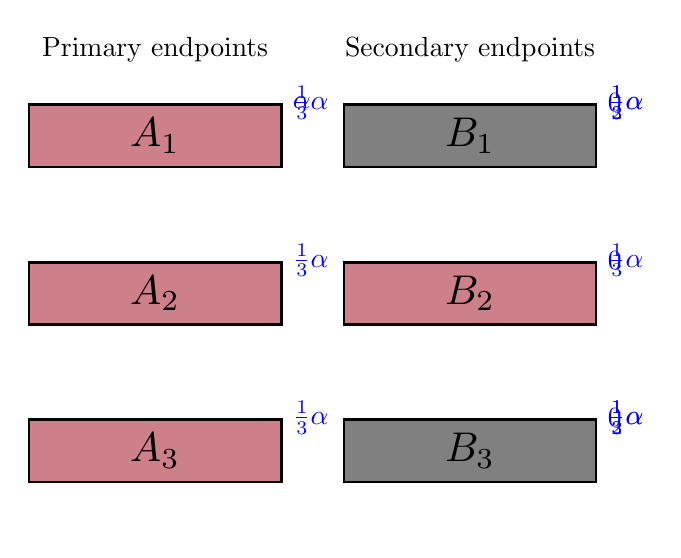
\begin{tikzpicture}
  \path (0,0) rectangle (7,6) ;
  \path<1-3> (1,5) node[draw, scale=1.5,  line width=1pt, text width=1.9cm, text centered, fill=cambridgedarkblue!50] (a1) {$A_1$} ;
  \path<4-> (1,5) node[draw, scale=1.5, line width=1pt, text width=1.9cm, text centered, fill=cambridgedarkorange!50] (a1) {$A_1$} ;
  \path<1-2> (a1.north east) node[anchor=west, blue] {$\frac13\alpha$} ;
  \path<3> (a1.north east) node[anchor=west, blue] {$\alpha$} ;

  \path<1> (1,3) node[draw, scale=1.5,  line width=1pt, text width=1.9cm, text centered, fill=cambridgedarkblue!50] (a2) {$A_2$} ;
  \path<2-> (1,3) node[draw, scale=1.5, line width=1pt, text width=1.9cm, text centered, fill=cambridgedarkorange!50] (a2) {$A_2$} ;
  \path<1> (a2.north east) node[anchor=west, blue] {$\frac13\alpha$} ;

  \path<1> (1,1) node[draw, scale=1.5,  line width=1pt, text width=1.9cm, text centered, fill=cambridgedarkblue!50] (a3) {$A_3$} ;
  \path<2-> (1,1) node[draw, scale=1.5, line width=1pt, text width=1.9cm, text centered, fill=cambridgedarkorange!50] (a3) {$A_3$} ;
  \path<1> (a3.north east) node[anchor=west, blue] {$\frac13\alpha$} ;

  \path<1-4> (5,5) node[draw, scale=1.5,  line width=1pt, text width=1.9cm, text centered] (b1) {$B_1$} ;
  \path<5-> (5,5) node[draw, scale=1.5,  line width=1pt, text width=1.9cm, text centered, fill=cambridgedarkblue!50] (b1) {$B_1$} ;
  \path<1-4> (b1.north east) node[anchor=west, blue] {$0$} ;
  \path<5-6> (b1.north east) node[anchor=west, blue] {$\frac13\alpha$} ;
  \path<7-> (b1.north east) node[anchor=west, blue] {$\frac12\alpha$} ;

  \path<1-4> (5,3) node[draw, scale=1.5,  line width=1pt, text width=1.9cm, text centered] (b2) {$B_2$} ;
  \path<5> (5,3) node[draw, scale=1.5,  line width=1pt, text width=1.9cm, text centered, fill=cambridgedarkblue!50] (b2) {$B_2$} ;
  \path<6-> (5,3) node[draw, scale=1.5, line width=1pt, text width=1.9cm, text centered, fill=cambridgedarkorange!50] (b2) {$B_2$} ;
  \path<1-4> (b2.north east) node[anchor=west, blue] {$0$} ;
  \path<5> (b2.north east) node[anchor=west, blue] {$\frac13\alpha$} ;

  \path<1-4> (5,1) node[draw, scale=1.5,  line width=1pt, text width=1.9cm, text centered] (b3) {$B_3$} ;
  \path<5-> (5,1) node[draw, scale=1.5,  line width=1pt, text width=1.9cm, text centered, fill=cambridgedarkblue!50] (b3) {$B_3$} ;
  \path<1-4> (b3.north east) node[anchor=west, blue] {$0$} ;
  \path<5-6> (b3.north east) node[anchor=west, blue] {$\frac13\alpha$} ;
  \path<7-> (b3.north east) node[anchor=west, blue] {$\frac12\alpha$} ;

  \path (1,6.1) node {Primary endpoints} ;
  \path (5,6.1) node {Secondary endpoints} ;
  \end{tikzpicture}
\end{figure}
\end{frame}


\bfr{Parallel gatekeeping}
\begin{overprint}
  \onslide<1>
    Test all primary endpoints at $\alpha/3$
  \onslide<2>
    If we reject a few\ldots
  \onslide<3>
    Go on with the secondary endpoints with the available $\alpha$
  \onslide<4>
    Suppose we are able to reject some of the secondary endpoints\ldots
  \onslide<5>
    Go on doing Holm for the secondary endpoints
  \onslide<6>
    And if we reject all secondary ones\ldots
  \onslide<7>
    Go on doing Holm for the primary endpoints
\end{overprint}
\begin{figure}
  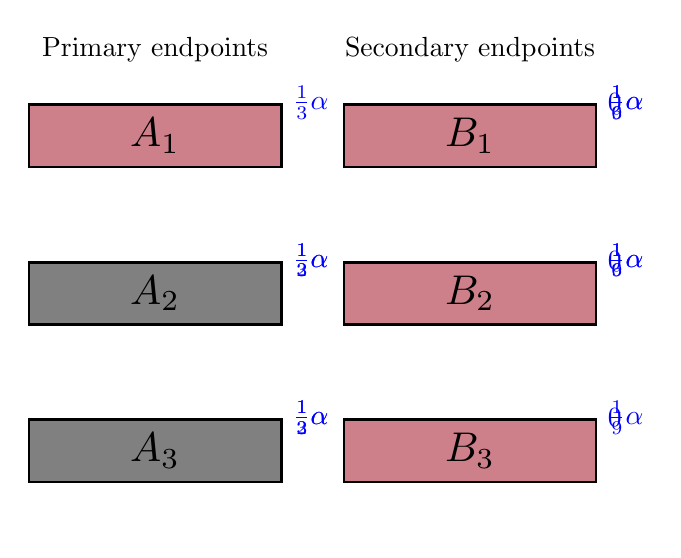
\begin{tikzpicture}
  \path (0,0) rectangle (7,6) ;
  \path<1> (1,5) node[draw, scale=1.5,  line width=1pt, text width=1.9cm, text centered, fill=cambridgedarkblue!50] (a1) {$A_1$} ;
  \path<2-> (1,5) node[draw, scale=1.5, line width=1pt, text width=1.9cm, text centered, fill=cambridgedarkorange!50] (a1) {$A_1$} ;
  \path<1> (a1.north east) node[anchor=west, blue] {$\frac13\alpha$} ;

  \path (1,3) node[draw, scale=1.5,  line width=1pt, text width=1.9cm, text centered, fill=cambridgedarkblue!50] (a2) {$A_2$} ;
  \path<1-6> (a2.north east) node[anchor=west, blue] {$\frac13\alpha$} ;
  \path<7-> (a2.north east) node[anchor=west, blue] {$\frac12\alpha$} ;

  \path (1,1) node[draw, scale=1.5,  line width=1pt, text width=1.9cm, text centered, fill=cambridgedarkblue!50] (a3) {$A_3$} ;
  \path<1-6> (a3.north east) node[anchor=west, blue] {$\frac13\alpha$} ;
  \path<7-> (a3.north east) node[anchor=west, blue] {$\frac12\alpha$} ;

  \path<1-2> (5,5) node[draw, scale=1.5,  line width=1pt, text width=1.9cm, text centered] (b1) {$B_1$} ;
  \path<3-5> (5,5) node[draw, scale=1.5,  line width=1pt, text width=1.9cm, text centered, fill=cambridgedarkblue!50] (b1) {$B_1$} ;
  \path<6-> (5,5) node[draw, scale=1.5, line width=1pt, text width=1.9cm, text centered, fill=cambridgedarkorange!50] (b1) {$B_1$} ;
  \path<1-2> (b1.north east) node[anchor=west, blue] {$0$} ;
  \path<3-4> (b1.north east) node[anchor=west, blue] {$\frac19\alpha$} ;
  \path<5> (b1.north east) node[anchor=west, blue] {$\frac16\alpha$} ;

  \path<1-2> (5,3) node[draw, scale=1.5,  line width=1pt, text width=1.9cm, text centered] (b2) {$B_2$} ;
  \path<3-5> (5,3) node[draw, scale=1.5,  line width=1pt, text width=1.9cm, text centered, fill=cambridgedarkblue!50] (b2) {$B_2$} ;
  \path<6-> (5,3) node[draw, scale=1.5, line width=1pt, text width=1.9cm, text centered, fill=cambridgedarkorange!50] (b2) {$B_2$} ;
  \path<1-2> (b2.north east) node[anchor=west, blue] {$0$} ;
  \path<3-4> (b2.north east) node[anchor=west, blue] {$\frac19\alpha$} ;
  \path<5> (b2.north east) node[anchor=west, blue] {$\frac16\alpha$} ;

  \path<1-2> (5,1) node[draw, scale=1.5,  line width=1pt, text width=1.9cm, text centered ] (b3) {$B_3$} ;
  \path<3> (5,1) node[draw, scale=1.5,  line width=1pt, text width=1.9cm, text centered, fill=cambridgedarkblue!50] (b3) {$B_3$} ;
  \path<4-> (5,1) node[draw, scale=1.5, line width=1pt, text width=1.9cm, text centered, fill=cambridgedarkorange!50] (b3) {$B_3$} ;
  \path<1-2> (b3.north east) node[anchor=west, blue] {$0$} ;
  \path<3> (b3.north east) node[anchor=west, blue] {$\frac19\alpha$} ;

  \path (1,6.1) node {Primary endpoints} ;
  \path (5,6.1) node {Secondary endpoints} ;
  \end{tikzpicture}
\end{figure}
\end{frame}


%%%%%%%%%%%%%%%%%%%%%%%%%%%%%%%%%%%%%%%%%%%%%%%%%%%%%%%%%%%%%%%%%%%%%%%%%%%%%%%%%%%%%%%%%%%%%%%%%%%%%%
\subsection{}
\begin{frame}
\frametitle{Example: clinical trial in patients with hypertension} 

\textcolor{cambridgedarkorange}{Study design:} two doses versus placebo

\bigskip

$\begin{array}{cl}
   X_{1},\ldots,X_{m}\stackrel{\mathrm{i.i.d.}}{\sim} N(\psi_x,1) & \mathrm{Placebo} \\ 
   Y_{1},\ldots,Y_{n}\stackrel{\mathrm{i.i.d.}}{\sim}N(\psi_y,1) &  \mathrm{Low\,\,dose}\\ 
   Z_{1},\ldots,Z_{n}\stackrel{\mathrm{i.i.d.}}{\sim}N(\psi_z,1) & \mathrm{High\,\,dose} \\
\end{array}$


\bigskip

\textcolor{cambridgedarkorange}{Primary endpoint:} reduction in diastolic blood pressure

\bigskip

$\begin{array}{ccc}
    A: \psi_x = \psi_y & \mathrm{versus} &  \tilde{A}:  \psi_x>\psi_y \\ 
    B: \psi_x = \psi_z & \mathrm{versus}   &  \tilde{B}: \psi_x>\psi_z\\ 
\end{array}$

\bigskip

\textcolor{cambridgedarkorange}{Statistics:} marginal and joint null distributions



\begin{columns}[t]
\column{0.45\textwidth}

$\begin{array}{c}
    S_A=\sqrt{\frac{mn}{m+n}}(\bar{X}-\bar{Y}) \stackrel{A}{\sim} N(0,1)\\ 
    S_B=\sqrt{\frac{mn}{m+n}}( \bar{X}-\bar{Z}) \stackrel{B}{\sim} N(0,1)\\ 
\end{array}$


\column{0.55\textwidth}


$$
\left(   \begin{array}{c}
    S_A \\ 
    S_B \\ 
\end{array}\right) \stackrel{A,B}{\sim} N_{2}\left(   
\left[\begin{array}{c}
    0 \\ 
    0 \\ 
\end{array}\right], \left[\begin{array}{cc}
    1 & \lambda \\ 
    \lambda & 1\\ 
\end{array}\right]  \right)$$

$\lambda= \frac{n}{n+m}\,\,$  nuisance parameter

\end{columns}


\end{frame}
%%%%%%%%%%%%%%%%%%%%%%%%%%%%%%%%%%%%%%%%%%%%%%%%%%%%%%%%%%%%%%%%%%%%%%%%%%%%%%%%%%%%%%%%%%%%%%%%%%%%%%
\subsection{}
\begin{frame}
\frametitle{Bonferroni's bound: positive dependence} 

$\mathrm{FWE}=\Pr\left(\left\{S_A > c \right\} \cup \left\{S_B > c \right\} \right)$ using $c=z_{1-\frac{\alpha}{2}}$ (Bonferroni) is equal

\smallskip

$$\underbrace{\Pr\left(S_A>  z_{1-\frac{\alpha}{2}} \right)}_{\alpha/2}+ \underbrace{\Pr\left(S_B >  z_{1-\frac{\alpha}{2}} \right)}_{\alpha/2}  -\underbrace{ \Pr\left(\left\{S_A >  z_{1-\frac{\alpha}{2}} \right\} \cap \left\{S_B >  z_{1-\frac{\alpha}{2}} \right\} \right)}_{\alpha(\lambda)}$$

\bigskip

\begin{columns}[t]

\column{0.45\textwidth}
\centering
\textcolor{cambridgedarkorange}{$n=3m$, $\lambda=3/4$, $\mathrm{FWE}=0.04$}\\
\includegraphics[scale=.33]{lambda75}

\column{0.45\textwidth}
\centering
\textcolor{cambridgedarkorange}{$0<\lambda<1$, $\uparrow$ dose levels}\\
\includegraphics[scale=.33]{lambdarho}
\end{columns}

\end{frame}
%%%%%%%%%%%%%%%%%%%%%%%%%%%%%%%%%%%%%%%%%%%%%%%%%%%%%%%%%%%%%%%%%%%%%%%%%%%%%%%%%%%%%%%%%%%%%%%%%%%%%%
\subsection{}
\begin{frame}
\frametitle{Bonferroni's bound: worst dependence case} 

\textcolor{cambridgedarkorange}{Two-sided testing}

\bigskip

$\begin{array}{ccc}
    A: \psi = 0 & \mathrm{versus} &  \tilde{A}:  \psi>0\\ 
    B: \psi = 0 & \mathrm{versus}   &  \tilde{B}: \psi<0\\ 
\end{array}$

\bigskip

\textcolor{cambridgedarkorange}{$S_{B}\equiv -S_A\Rightarrow \lambda = -1$ (disjoint rejection regions)}
\begin{eqnarray*}
\mathrm{FWE}=\Pr\left(S_A > z_{1-\frac{\alpha}{2}} \right) + \Pr\left(-S_A > z_{1-\frac{\alpha}{2}} \right) = \alpha
% &=&\Pr\left(S_A < z_{\frac{\alpha}{2}} \right) + \Pr\left(S_A > z_{1-\frac{\alpha}{2}} \right) =\alpha
\end{eqnarray*}

\begin{columns}[t]

\column{0.45\textwidth}
\centering
\includegraphics[scale=.32]{lambda_1}

\column{0.45\textwidth}
\centering
\includegraphics[scale=.32]{lambda_1b}
\end{columns}


\end{frame}
%%%%%%%%%%%%%%%%%%%%%%%%%%%%%%%%%%%%%%%%%%%%%%%%%%%%%%%%%%%%%%%%%%%%%%%%%%%%%%%%%%%%%%%%%%%%%%%%%%%%%%
\subsection{}
\begin{frame}
\frametitle{Stepdown $S_{\max}$ (parametric)} 

Make use of the dependence structure of test statistics

\begin{columns}[t]

\column{0.5\textwidth}

\textcolor{cambridgedarkorange}{\textbf{Stepdown procedure}}


\begin{enumerate}
\item Find the null distribution of $S_{\max}=\max_{H\in \mathcal{H}}(S_H)$
\item Reject $H$ if $S_{H}>c_{1-\alpha}$,\\ the $(1-\alpha)$-quantile of $\mathrm{d}_{S_{\max}}$
\item Recompute the distribution of $S_{\max}=\max_{H\in \mathcal{H}\setminus \mathcal{R}  }(S_H)$
\item Repeat
\end{enumerate}

\column{0.55\textwidth}

\only<1>{\textcolor{cambridgedarkorange}{Find $c_{1-\alpha}$ from $\mathrm{d}_{S_{\max}}=\mathrm{d}_{\max(S_A,S_B)}$ }}
\only<2>{\textcolor{cambridgedarkorange}{Suppose $S_B > c_{1-\alpha}$}}
\only<3>{\textcolor{cambridgedarkorange}{Find $z_{1-\alpha}$ from $\mathrm{d}_{S_{\max}}=\mathrm{d}_{S_A}$}}
\only<4>{\textcolor{cambridgedarkorange}{Suppose $S_{A} > z_{1-\alpha}$}}

\begin{tikzpicture}
\node at (-.4,.5) {$\mathcal{H}\setminus \mathcal{R}:$};
\node at (0,0) {$\mathcal{R}:$};
\only<1>{
\node at (1,1) {$c_{1-\alpha}$};
\node at (2,1) {$c_{1-\alpha}$};
\draw[] 
(1,.5) node[draw, line width=1pt,fill=cambridgedarkblue!50] {A}
(2,.5) node[draw, line width=1pt,fill=cambridgedarkblue!50] {B};}
\only<2>{
\node at (1,1) {$c_{1-\alpha}$};
\node at (2,1) {$c_{1-\alpha}$};
\draw[] 
(1,.5) node[draw, line width=1pt,fill=cambridgedarkblue!50] {A}
(2,.5) node[draw, line width=1pt,fill=cambridgedarkorange!50] {B};}
\only<3>{
\node at (1,1) {$z_{1-\alpha}$};
\node at (2,1) {$-$};
\draw[] 
(1,.5) node[draw, line width=1pt,fill=cambridgedarkblue!50] {A}
(2,0) node[draw, line width=1pt,fill=cambridgedarkorange!50] {B};}
\only<4>{
\node at (1,1) {$-$};
\node at (2,1) {$-$};
\draw[] 
(1,0) node[draw, line width=1pt,fill=cambridgedarkorange!50] {A}
(2,0) node[draw, line width=1pt,fill=cambridgedarkorange!50] {B};}
\end{tikzpicture}



\only<1-2>{\includegraphics[scale=.33]{step1}}
\only<3->{\includegraphics[scale=.33]{step2}}


\end{columns}

\end{frame}
%%%%%%%%%%%%%%%%%%%%%%%%%%%%%%%%%%%%%%%%%%%%%%%%%%%%%%%%%%%%%%%%%%%%%%%%%%%%%%%%%%%%%%%%%%%%%%%%%%%%%%
\subsection{}
\begin{frame}
\frametitle{Stepdown $S_{\max}$ (resampling based)} 

Make use of the dependence structure of test statistics

\begin{columns}[t]

\column{0.5\textwidth}

\textcolor{cambridgedarkorange}{\textbf{Stepdown procedure}}


\begin{enumerate}
\item Find the null distribution$^{*}$ of $S_{\max}=\max_{H\in \mathcal{H}}(S_H)$
\item Reject $H$ if $S_{H}>c^{*}_{1-\alpha}$,\\ the $(1-\alpha)$-quantile of $\mathrm{d}^{*}_{S_{\max}}$
\item Recompute the distribution$^{*}$ of $S_{\max}=\max_{H\in \mathcal{H}\setminus \mathcal{R}  }(S_H)$
\item Repeat
\end{enumerate}

$^{*}$ bootstrap (parametric and non-), permutations 

\bigskip
\textcolor{cambridgedarkorange}{Assumption:} 
 "subset pivotality", exchangeability

\column{0.55\textwidth}

\only<1>{\textcolor{cambridgedarkorange}{Find $c^{*}_{1-\alpha}$ from $\mathrm{d}^{*}_{S_{\max}}=\mathrm{d}^{*}_{\max(S_A,S_B)}$}}
\only<2>{\textcolor{cambridgedarkorange}{Suppose $S_B > c^{*}_{1-\alpha}$}}
\only<3>{\textcolor{cambridgedarkorange}{Find $z^{*}_{1-\alpha}$ from $\mathrm{d}^{*}_{S_{\max}}=\mathrm{d}^{*}_{S_A}$}}
\only<4>{\textcolor{cambridgedarkorange}{Suppose $S_{A} \leq z^{*}_{1-\alpha}$. Stop}}

\begin{tikzpicture}
\node at (-.4,.5) {$\mathcal{H}\setminus \mathcal{R}:$};
\node at (0,0) {$\mathcal{R}:$};
\only<1>{
\node at (1,1) {$c^{*}_{1-\alpha}$};
\node at (2,1) {$c^{*}_{1-\alpha}$};
\draw[] 
(1,.5) node[draw, line width=1pt,fill=cambridgedarkblue!50] {A}
(2,.5) node[draw, line width=1pt,fill=cambridgedarkblue!50] {B};}
\only<2>{
\node at (1,1) {$c^{*}_{1-\alpha}$};
\node at (2,1) {$-$};
\draw[] 
(1,.5) node[draw, line width=1pt,fill=cambridgedarkblue!50] {A}
(2,0) node[draw, line width=1pt,fill=cambridgedarkorange!50] {B};}
\only<3>{
\node at (1,1) {$z^{*}_{1-\alpha}$};
\node at (2,1) {$-$};
\draw[] 
(1,.5) node[draw, line width=1pt,fill=cambridgedarkblue!50] {A}
(2,0) node[draw, line width=1pt,fill=cambridgedarkorange!50] {B};}
\only<4>{
\node at (1,1) {$z^{*}_{1-\alpha}$};
\node at (2,1) {$-$};
\draw[] 
(1,.5) node[draw, line width=1pt,fill=cambridgedarkblue!50] {A}
(2,0) node[draw, line width=1pt,fill=cambridgedarkorange!50] {B};}
\end{tikzpicture}



\only<1-2>{\includegraphics[scale=.33]{step1R}}
\only<3->{\includegraphics[scale=.33]{step2R}}


\end{columns}

\end{frame}



%%%%%%%%%%%%%%%%%%%%%%%%%%%%%%%%%%%%%%%%%%%%%%%%%%%%%%%%%%%%%%%%%%%%%%%%%%%%%%%%%%%%%%%%%%%%%%%%%%%%%%
\section{The sequential rejection principle}
\subsection{}
\begin{frame}
\frametitle{All similar methods}


\begin{enumerate}
\item Start testing hypotheses at some significance criterion
\item If any hypotheses rejected, set new significance criterion for unrejected hypotheses
\item Possibly new rejections
\item Stop if no new rejections occur
\end{enumerate}

\bigskip
\textcolor{cambridgedarkorange}{Are these all examples of the same procedure?}
\bigskip


\textcolor{cambridgedarkorange}{\textbf{The general procedure}}

\bigskip


$\mathcal{R}_{i}\subseteq \mathcal{H}$: the rejected hypotheses after step $i$

\begin{eqnarray*}
\mathcal{R}_{0} &=& \emptyset\\
\mathcal{R}_{i+1} &=& \mathcal{R}_{i} \cup \{H \in \mathcal{H}: S_{H} > c_H(\mathcal{R}_{i})\} 
\end{eqnarray*}

After every step the procedure adjusts the critical values on the basis of the new rejected set

\end{frame}
%%%%%%%%%%%%%%%%%%%%%%%%%%%%%%%%%%%%%%%%%%%%%%%%%%%%%%%%%%%%%%%%%%%%%%%%%%%%%%%%%%%%%%%%%%%%%%%%%%%%%%
\subsection{}
\begin{frame}
\frametitle{The Sequential Rejection Principle}



\textcolor{cambridgedarkorange}{\textbf{Theorem}\footnote{J.J. Goeman and A. Solari (2008) The sequential rejection principle of familywise error control. \emph{Submitted}}}

\bigskip
If a general sequentially rejective procedure fulfills two conditions
\begin{enumerate}
\item Monotonicity
\item Single step control
\end{enumerate}
Then it controls the FWE

\bigskip

\only<1>{
\textcolor{cambridgedarkorange}{Monotonicity condition:}
for every $\mathcal{S}\subseteq \mathcal{R}\subset\mathcal{H}$ and every $H\in \mathcal{H}\setminus\mathcal{R}$,

$$c_{H}(\mathcal{S})\geq c_{H}(\mathcal{R})$$

\textcolor{cambridgedarkorange}{In words:}
critical values of unrejected null hypotheses never increase with
more rejections

\textcolor{cambridgedarkorange}{Note:} monotonicity implies $c_{H}(\mathcal{R}_{i})\geq c_{H}(\mathcal{R}_{i+1})$, but this is too weak to guarantee FWE control
}
\only<2>{
\textcolor{cambridgedarkorange}{Single step condition:}
for every $\mathcal{R}\subset\mathcal{H}$ and $\mathcal{T}=\mathcal{H}\setminus \mathcal{R}$,

$$\Pr\left(\bigcup_{H\in \mathcal{T}} \left\{S_H > c_H(\mathcal{R})\right\}\right)\leq \alpha$$

\textcolor{cambridgedarkorange}{In words:}
FWE weak control is guaranteed at each single step.\\
It may be assumed that all previous rejections were correct
rejections
}


% \only<3>{
% \textcolor{cambridgedarkorange}{Proof:}
% \begin{itemize}
% \item `Worst case': all false null hypotheses have been rejected
% \item Single step condition guarantees FWE control in the worst case
% \item Monotonicity guarantees: no false rejections in the worst case implies no false rejections `on the way' to the worst case 
% \end{itemize}
% }

\only<4>{
\textcolor{cambridgedarkorange}{A unifying approach:}
\begin{itemize}
\item Facilitates formulation of FWE controlling procedures
\item Facilitates proof of FWE control
\item Makes connections between methods more obvious 
\end{itemize}
}

\end{frame}

%%%%%%%%%%%%%%%%%%%%%%%%%%%%%%%%%%
%%%%%%%%%%%%%%%%%%%%%%%%%%%%%%%%%%%%%%%%%%%%%%%%%%%%%%%%%%%%%%%%%%%%%%%%%%%%%%%%%%%%%%%%%%%%%%%%%%%%%%
%%%%%%%%%%%%%%%%%%%%%%%%%%%%%%%%%%%%%%%%%55
\section{Inheritance procedure}

\bfr{Problems with a natural tree structure}
  \bb{Genetic association studies}
      -$\circ$ Whole genome
    \\---$\circ$ chromosomes
    \\-----$\circ$ genes
  \eb
  \pause
  \bb{Self Report psychological/sociological questionnaires}
      -$\circ$ investigated concepts
    \\---$\circ$ different aspects
    \\-----$\circ$ single items (questions)
  \eb
  \pause
  \bb{Alternative}
    Make a tree structure from the data by hierarchical clustering
  \eb
\end{frame}




% ==========================
\begin{frame}
\frametitle{Example of Tree-Structured Hypotheses: Genes}

%\begin{figure}
\begin{center}
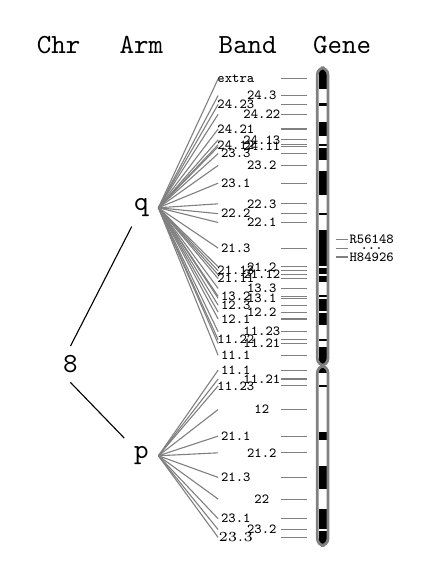
\begin{tikzpicture}
\begin{scope}[scale=.15,yshift=-6cm, font=\ttfamily]

\path  (-4,42.25) node {Chr};			
\path  (3,42.25) node {Arm};			
\path  (12,42.25) node {Band};			
\path  (20,42.25) node {Gene};			
\path  (-3,15.25) node (ch8) { 8};	
\path  (3,7.5) node (p) {p}; \draw  (ch8.south) -- (p);
\path  (3,28.5) node (q) { q};\draw  (ch8.north) -- (q);

\fill		(18,0) rectangle +(.7,1.17);	\path  (11,0.58) node (n1) {\tiny $23.3$} ;
\draw[color=gray]  (14.8,0.583333333333333) -- (17,0.583333333333333);
\draw[color=gray]  (p.east) -- (9.5,0.583333333333333);
\fill	[color=white]	(18,1.17) rectangle +(.7,0.17);	\path  (13.2,1.25) node (n2) {\tiny 23.2} ;
\draw[color=gray]  (14.8,1.25) -- (17,1.25); \draw[color=gray]  (p.east) -- (9.5,1.25);
\fill		(18,1.33) rectangle +(.7,1.67);	\path  (11,2.17) node (n3) {\tiny 23.1} ;
\draw[color=gray]  (14.8,2.16666666666667) -- (17,2.16666666666667); 
\draw[color=gray]  (p.east) -- (9.5,2.16666666666667);
\fill	[color=white]	(18,3) rectangle +(.7,1.67);	\path  (13.2,3.83) node (n4) {\tiny 22} ;
\draw[color=gray]  (14.8,3.83333333333333) -- (17,3.83333333333333); 
\draw[color=gray]  (p.east) -- (9.5,3.83333333333333);
\fill		(18,4.67) rectangle +(.7,2);	\path  (11,5.67) node (n5) {\tiny 21.3} ;
\draw[color=gray]  (14.8,5.66666666666667) -- (17,5.66666666666667);
 \draw[color=gray]  (p.east) -- (9.5,5.66666666666667);
\fill	[color=white]	(18,6.67) rectangle +(.7,2.17);	\path  (13.2,7.75) node (n6) {\tiny 21.2} ;
\draw[color=gray]  (14.8,7.75) -- (17,7.75); \draw[color=gray]  (p.east) -- (9.5,7.75);
\fill		(18,8.83) rectangle +(.7,0.67);	\path  (11,9.17) node (n7) {\tiny 21.1} ;
\draw[color=gray]  (14.8,9.16666666666667) -- (17,9.16666666666667); 
\draw[color=gray]  (p.east) -- (9.5,9.16666666666667);
\fill	[color=white]	(18,9.5) rectangle +(.7,3.83);	\path  (13.2,11.42) node (n8) {\tiny 12} ;
\draw[color=gray]  (14.8,11.4166666666667) -- (17,11.4166666666667);
 \draw[color=gray]  (p.east) -- (9.5,11.4166666666667);
\fill		(18,13.33) rectangle +(.7,0.17);	\path  (11,13.42) node (n9) {\tiny 11.23} ;
\draw[color=gray]  (14.8,13.4166666666667) -- (17,13.4166666666667); 
\draw[color=gray]  (p.east) -- (9.5,13.4166666666667);
\fill	[color=white]	(18,13.5) rectangle +(.7,1);	\path  (13.2,14) node (n10) {\tiny 11.21} ;
\draw[color=gray]  (14.8,14) -- (17,14); \draw[color=gray]  (p.east) -- (9.5,14);
\fill		(18,14.5) rectangle +(.7,0.5);	\path  (11,14.75) node (n11) {\tiny 11.1} ;
\draw[color=gray]  (14.8,14.75) -- (17,14.75); \draw[color=gray]  (p.east) -- (9.5,14.75);			
\fill		(18,15.25) rectangle +(.7,1.5);	\path  (11,16) node (n13) {\tiny 11.1} ;
\draw[color=gray]  (14.8,16) -- (17,16); \draw[color=gray]  (q.east) -- (9.5,16);
\fill	[color=white]	(18,16.75) rectangle +(.7,0.5);	\path  (13.2,17) node (n14) {\tiny 11.21} ;
\draw[color=gray]  (14.8,17) -- (17,17); \draw[color=gray]  (q.east) -- (9.5,17);
\fill		(18,17.25) rectangle +(.7,0.17);	\path  (11,17.33) node (n15) {\tiny 11.22} ;
\draw[color=gray]  (14.8,17.3333333333333) -- (17,17.3333333333333); 
\draw[color=gray]  (q.east) -- (9.5,17.3333333333333);
\fill	[color=white]	(18,17.42) rectangle +(.7,1.17);	\path  (13.2,18) node (n16) {\tiny 11.23} ;
\draw[color=gray]  (14.8,18) -- (17,18); \draw[color=gray]  (q.east) -- (9.5,18);
\fill		(18,18.58) rectangle +(.7,1);	\path  (11,19.08) node (n17) {\tiny 12.1} ;
\draw[color=gray]  (14.8,19.0833333333333) -- (17,19.0833333333333); 
\draw[color=gray]  (q.east) -- (9.5,19.0833333333333);
\fill	[color=white]	(18,19.58) rectangle +(.7,0.17);	\path  (13.2,19.67) node (n18) {\tiny 12.2} ;
\draw[color=gray]  (14.8,19.6666666666667) -- (17,19.6666666666667); 
\draw[color=gray]  (q.east) -- (9.5,19.6666666666667);
\fill		(18,19.75) rectangle +(.7,1);	\path  (11,20.25) node (n19) {\tiny 12.3} ;
\draw[color=gray]  (14.8,20.25) -- (17,20.25); \draw[color=gray]  (q.east) -- (9.5,20.25);
\fill	[color=white]	(18,20.75) rectangle +(.7,0.17);	\path  (13.2,20.83) node (n20) {\tiny 13.1} ;
\draw[color=gray]  (14.8,20.8333333333333) -- (17,20.8333333333333);
 \draw[color=gray]  (q.east) -- (9.5,20.8333333333333);
\fill		(18,20.92) rectangle +(.7,0.17);	\path  (11,21) node (n21) {\tiny 13.2} ;
\draw[color=gray]  (14.8,21) -- (17,21); 
\draw[color=gray]  (q.east) -- (9.5,21);
\fill	[color=white]	(18,21.08) rectangle +(.7,1.17);	\path  (13.2,21.67) node (n22) {\tiny 13.3} ;
\draw[color=gray]  (14.8,21.6666666666667) -- (17,21.6666666666667);
 \draw[color=gray]  (q.east) -- (9.5,21.6666666666667);
\fill		(18,22.25) rectangle +(.7,0.5);	\path  (11,22.5) node (n23) {\tiny 21.11} ;
\draw[color=gray]  (14.8,22.5) -- (17,22.5); 
\draw[color=gray]  (q.east) -- (9.5,22.5);
\fill	[color=white]	(18,22.75) rectangle +(.7,0.17);	\path  (13.2,22.83) node (n24) {\tiny 21.12} ;
\draw[color=gray]  (14.8,22.8333333333333) -- (17,22.8333333333333); 
\draw[color=gray]  (q.east) -- (9.5,22.8333333333333);
\fill		(18,22.92) rectangle +(.7,0.5);	\path  (11,23.17) node (n25) {\tiny 21.13} ;
\draw[color=gray]  (14.8,23.1666666666667) -- (17,23.1666666666667); 
\draw[color=gray]  (q.east) -- (9.5,23.1666666666667);
\fill	[color=white]	(18,23.42) rectangle +(.7,0.17);	\path  (13.2,23.5) node (n26) {\tiny 21.2} ;
\draw[color=gray]  (14.8,23.5) -- (17,23.5); \draw[color=gray]  (q.east) -- (9.5,23.5);
\fill		(18,23.58) rectangle +(.7,3);	\path  (11,25.08) node (n27) {\tiny  21.3} ;
\draw[color=gray]  (14.8,25.0833333333333) -- (17,25.0833333333333); 
\draw[color=gray]  (q.east) -- (9.5,25.0833333333333);
\fill	[color=white]	(18,26.58) rectangle +(.7,1.33);	\path  (13.2,27.25) node (n28) {\tiny 22.1} ;
\draw[color=gray]  (14.8,27.25) -- (17,27.25); 
\draw[color=gray]  (q.east) -- (9.5,27.25);
\fill		(18,27.92) rectangle +(.7,0.17);	\path  (11,28) node (n29) {\tiny 22.2} ;
\draw[color=gray]  (14.8,28) -- (17,28); 
\draw[color=gray]  (q.east) -- (9.5,28);
\fill	[color=white]	(18,28.08) rectangle +(.7,1.5);	\path  (13.2,28.83) node (n30) {\tiny 22.3} ;
\draw[color=gray]  (14.8,28.8333333333333) -- (17,28.8333333333333); 
\draw[color=gray]  (q.east) -- (9.5,28.8333333333333);
\fill		(18,29.58) rectangle +(.7,2);	\path  (11,30.58) node (n31) {\tiny 23.1} ;
\draw[color=gray]  (14.8,30.5833333333333) -- (17,30.5833333333333); 
\draw[color=gray]  (q.east) -- (9.5,30.5833333333333);
\fill	[color=white]	(18,31.58) rectangle +(.7,1);	\path  (13.2,32.08) node (n32) {\tiny 23.2} ;
\draw[color=gray]  (14.8,32.0833333333333) -- (17,32.0833333333333); 
\draw[color=gray]  (q.east) -- (9.5,32.0833333333333);
\fill		(18,32.58) rectangle +(.7,1);	\path  (11,33.08) node (n33) {\tiny 23.3} ;
\draw[color=gray]  (14.8,33.0833333333333) -- (17,33.0833333333333); 
\draw[color=gray]  (q.east) -- (9.5,33.0833333333333);
\fill	[color=white]	(18,33.58) rectangle +(.7,0.17);	\path  (13.2,33.67) node (n34) {\tiny 24.11} ;
\draw[color=gray]  (14.8,33.6666666666667) -- (17,33.6666666666667); 
\draw[color=gray]  (q.east) -- (9.5,33.6666666666667);
\fill		(18,33.75) rectangle +(.7,0.17);	\path  (11,33.83) node (n35) {\tiny 24.12} ;
\draw[color=gray]  (14.8,33.8333333333333) -- (17,33.8333333333333); 
\draw[color=gray]  (q.east) -- (9.5,33.8333333333333);
\fill	[color=white]	(18,33.92) rectangle +(.7,0.67);	\path  (13.2,34.25) node (n36) {\tiny 24.13} ;
\draw[color=gray]  (14.8,34.25) -- (17,34.25); \draw[color=gray]  (q.east) -- (9.5,34.25);
\fill		(18,34.58) rectangle +(.7,1.17);	\path  (11,35.17) node (n37) {\tiny 24.21} ;
\draw[color=gray]  (14.8,35.1666666666667) -- (17,35.1666666666667); 
\draw[color=gray]  (q.east) -- (9.5,35.1666666666667);
\fill	[color=white]	(18,35.75) rectangle +(.7,1.33);	\path  (13.2,36.42) node (n38) {\tiny 24.22} ;
\draw[color=gray]  (14.8,36.4166666666667) -- (17,36.4166666666667); 
\draw[color=gray]  (q.east) -- (9.5,36.4166666666667);
\fill		(18,37.08) rectangle +(.7,0.33);	\path  (11,37.25) node (n39) {\tiny 24.23} ;
\draw[color=gray]  (14.8,37.25) -- (17,37.25); \draw[color=gray]  (q.east) -- (9.5,37.25);
\fill	[color=white]	(18,37.42) rectangle +(.7,1.17);	\path  (13.2,38) node (n40) {\tiny 24.3} ;
\draw[color=gray]  (14.8,38) -- (17,38); \draw[color=gray]  (q.east) -- (9.5,38);
\fill		(18,38.58) rectangle +(.7,1.67);	\path  (11,39.42) node (n) {\tiny extra} ;
\draw[color=gray]  (14.8,39.4166666666667) -- (17,39.4166666666667); 
\draw[color=gray]  (q.east) -- (9.5,39.4166666666667);

\draw [color=gray, rounded corners=2.5pt, line width=1pt](17.9,-.1) rectangle (18.8,15.1);			
\draw [color=gray, rounded corners=2.5pt, line width=1pt](17.9,15.15) rectangle (18.8,40.35);			

\path (22.5,24.3333333333333) node {\tiny H84926}; \draw[color=gray]  (19.5,24.3333333333333) -- (20.5,24.3333333333333);			
\path (22.5,25.0833333333333) node {\tiny  ...}; \draw[color=gray]  (19.5,25.0833333333333) -- (20.5,25.0833333333333);			
\path (22.5,25.8333333333333) node {\tiny  R56148}; \draw[color=gray]  (19.5,25.8333333333333) -- (20.5,25.8333333333333);			
\end{scope}
\end{tikzpicture}
  \end{center}
\end{frame}

%% ==========================
\subsection{}
\bfr{}

\begin{figure}
  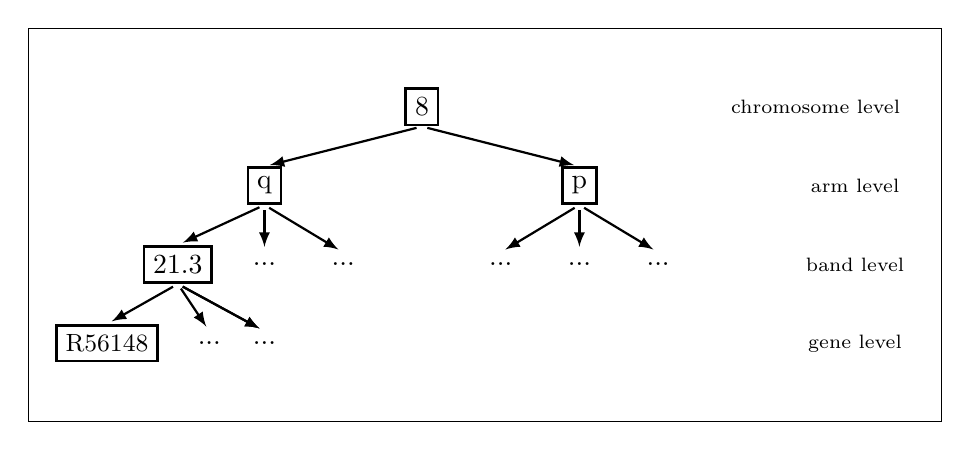
\begin{tikzpicture}
  \draw (0,-1) rectangle (11.6,4);
  \begin{scope}[draw, line width=1pt]
  \path          (5,3) node[draw] (top) {8} ;
  \path     (3,2)  node[draw] (abc) {q} ;
  \path    (7,2) node[draw] (de) {p} ;
  \path     (1.9,1) node[draw] (ab) {21.3} ;
  \path     (4,1) node[] (c) {...} ;
    \path     (3,1) node[] (h) {...} ;
  \path          (6,1) node[] (d) {...} ;
    \path          (7,1) node[] (f) {...} ;
  \path           (8,1) node[] (e) {...} ;
  \path     (1,0) node[draw] (a) {\small R56148};
    \path     (2.3,0) node[] (g) {...};
  \path            (3,0) node[] (b) {...};
    \path     (10.5,0)  node {{\scriptsize gene level}};
  \path     (10.5,1) node {{\scriptsize band level}};
  \path     (10.5,2)  node {{\scriptsize arm level}};
    \path     (10,3) node {{\scriptsize chromosome level}};
   \end{scope}
  \begin{scope}[thick, shorten >= 2pt,shorten <= 2pt, latex-]
    \draw         (abc.north) -- (top.south);
    \draw         (de.north) -- (top.south);
    \draw         (ab.north) -- (abc.south);
        \draw         (h.north) -- (abc.south);
    \draw (c.north) -- (abc.south);
    \draw (b.north) -- (ab.south);
    \draw (a.north) -- (ab.south);
    \draw (b.north) -- (ab.south);
        \draw (g.north) -- (ab.south);
    \draw (e.north) -- (de.south);
    \draw (d.north) -- (de.south);
       \draw (f.north) -- (de.south);
  \end{scope}
  \end{tikzpicture}
\end{figure}

\begin{overprint}

\onslide<1>
\begin{center}
root = general question, $\downarrow$ = more specific follow-up questions\\
\end{center}

\onslide<2>
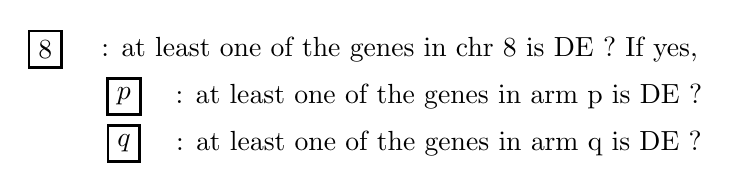
\begin{tikzpicture} \begin{scope}[draw, line width=1pt] 
\path (0,0)  node[draw] (a) {$8$};
\path (4.5,0)  node (a) {: at least one of the genes in chr 8 is DE ? If yes, };
\path (1,-.6)  node[draw] (a) {$p$};
\path (5,-.6)  node (a) {: at least one of the genes in arm p is DE ?};
\path (1,-1.2)  node[draw] (a) {$q$};
\path (5,-1.2)  node (a) {: at least one of the genes in arm q is DE ?};
 \end{scope} 
 \end{tikzpicture}
etc.

\end{overprint}

\end{frame}
% %% ==========================INHERITANCE
% \section{Inheritance procedure}
% \subsection{}
% 
% \begin{frame}
% \frametitle{Meinshausen's procedure (BMK 2008)}
% 
% \begin{overprint}
% 
%  \onslide<1>
%  
%  \bb{}{
%    start from the top: \\
%    test $ABCDE$ at level $\alpha$}\eb
%   \onslide<2>
%    \bb{}{
%    suppose $p_{ABCDE}\leq \alpha$, \\
%    test $ABC$ at $\frac{3}{5}\alpha$ and $DE$ at $\frac{2}{5} \alpha$}\eb
%    \onslide<3>
%     \bb{}{
%    suppose $p_{ABC}\leq \frac{3}{5}\alpha$ and $p_{DE}>\frac{2}{5} \alpha$}\eb
%    \onslide<4>
%     \bb{}{
%    test $AB$ at $\frac{2}{5}\alpha$ and $C$ at $\frac{1}{5}\alpha$}\eb
%    \onslide<5>
%     \bb{}{
%    suppose $p_{AB}\leq \frac{2}{5}\alpha$ and $p_{C}> \frac{1}{5}\alpha$, \\
%    test $A$ at  $\frac{1}{5}\alpha$ and $B$ at $\frac{1}{5}\alpha$}\eb
%    \onslide<6>
%     \bb{}{
%    suppose $p_{A}\leq \frac{1}{5}\alpha$ and $\frac{1}{5}\alpha < p_{B}< \frac{2}{5}\alpha$\\
%    STOP?}\eb
%   \onslide<7>
%       \bb{}{
%     \textcolor{green}{Shaffer's improvement:} if $A\cap B$ is a correct rejection, \\ at least one hypothesis is false: test $A$ and $B$ at level $\frac{2}{5}\alpha$
% }\eb
%   \onslide<8>
%       \bb{}{
%     reject A and B. \\
%     STOP!}\eb
% \end{overprint}
% 
% \begin{figure}
%   \begin{tikzpicture}
%   \draw (0,-1) rectangle (10,4);
%   \begin{scope}[draw, line width=1pt]
%     \path<1>   [blue]       (5,3) node[draw] (top) {$ABCDE$} ;
%   \path<1>[blue]    (top.east)   node {$\quad \alpha$} ;
%   \path<2>[blue] (5,3) node[draw] (top) {$ABCDE$} ;
%   \path<2->[red] (5,3) node[draw, cross out] (top) {$ABCDE$} ;
%   \path<2->[red] (5,3) node[draw] (top) {$ABCDE$} ;
%   \path<1-2>     (3,2)  node[draw] (abc) {$ABC$} ;
%   \path<2>[blue] (3,2)  node[draw] (abc) {$ABC$} ;
%   \path<2>[blue] (abc.east)  node {$\ \quad \alpha \frac{3}{5}$} ;
%   \path<3->[red] (3,2) node[draw, cross out] (abc) {$ABC$} ;
%   \path<3->[red] (3,2) node[draw] (abc) {$ABC$} ;
%   \path<1-2>     (7,2) node[draw] (de) {$DE$} ;
%   \path<2->[blue] (7,2) node[draw] (de) {$DE$} ;
%   \path<2->[blue] (de.east) node {$\ \quad \alpha \frac{2}{5}$} ;
%   \path<1-3>     (1.9,1) node[draw] (ab) {$AB$} ;
%   \path<4>[blue] (1.9,1) node[draw] (ab) {$AB$} ;
%   \path<4>[blue] (ab.east) node {$\ \quad  \alpha \frac{2}{5}$} ;
%   \path<5->[red] (1.9,1) node[draw, cross out] {$AB$} ;
%   \path<5->[red] (1.9,1) node[draw] {$AB$} ;
%   \path<1-3>     (4,1) node[draw] (c) {$C$} ;
%   \path<4->[blue] (4,1) node[draw] (c) {$C$} ;
%   \path<4->[blue] (c.east) node {$\ \quad \alpha \frac{1}{5}$} ;
%   \path          (6,1) node[draw] (d) {$D$} ;
%   \path           (8,1) node[draw] (e) {$E$} ;
%   \path     (1,0) node[draw] (a) {$A$};
%   \path<5>[blue] (1,0) node[draw] (a) {$A$};
%   \path<6>[red]  (1,0) node[draw] (a) {$A$};
%   \path<6>[red]  (1,0) node[draw, cross out] (a) {$A$};
%   \path<7>[blue] (1,0) node[draw] (a) {$A$};
%   \path<8>[red]  (1,0) node[draw] (a) {$A$};
%   \path<8>[red]  (1,0) node[draw, cross out] (a) {$A$};
%   \path<5>[blue] (a.east)node {$\ \quad \alpha \frac{1}{5}$} ;
%   \path<7>[green](a.east)node[draw] {$\ \quad \alpha \frac{2}{5}$} ;
%   \path            (3,0) node[draw] (b) {$B$};
%   \path<5->[blue]   (3,0) node[draw] (b) {$B$};
%   \path<5-6>[blue]  (b.east) node {$\ \quad \alpha \frac{1}{5}$} ;
%   \path<7>[green]    (b.east)node[draw] {$\ \quad  \alpha \frac{2}{5}$} ;
%   \path<8->[red]    (3,0) node[draw] (b) {$B$};
%   \path<8->[red]    (3,0) node[draw, cross out] (b) {$B$};
%   \end{scope}
%   \begin{scope}[thick, shorten >= 2pt,shorten <= 2pt, latex-]
%     \draw         (abc.north) -- (top.south);
%     \draw<2->[red] (abc.north) -- (top.south);
%     \draw         (de.north) -- (top.south);
%     \draw<2>[red] (de.north) -- (top.south);
%     \draw         (ab.north) -- (abc.south);
%     \draw<4->[red] (ab.north) -- (abc.south);
%     \draw (c.north) -- (abc.south);
%     \draw<4>[red] (c.north) -- (abc.south);
%     \draw (b.north) -- (ab.south);
%     \draw (a.north) -- (ab.south);
%     \draw (b.north) -- (ab.south);
%     \draw<5-6, 8>[red] (a.north) -- (ab.south);
%     \draw<5>[red] (b.north) -- (ab.south);
%         \draw<7>[green] (a.north) -- (ab.south);
%     \draw<7>[green] (b.north) -- (ab.south);
%         \draw<8>[red] (b.north) -- (ab.south);
%     \draw<4->[red] (d.north) -- (de.south);
%     \draw (e.north) -- (de.south);
%     \draw (d.north) -- (de.south);
%   \end{scope}
%   \end{tikzpicture}
% \end{figure}
% \end{frame}
%%%%%%%%%%%%%%%%%%%%%%%%%%%
% 
% %% ==========================================================
% \section{Tree structure}
% \subsection{}
% \begin{frame}
% \frametitle{Question(s)}
% 
% 
% \begin{overprint}
% 
% \onslide<1>
% \[
% \textcolor{white}{ h_i(y) = h(y)\exp(\mathbf{x}_{i}^{_{'}}\cdot \beta + z_i \lambda) }
% \]
% \begin{tikzpicture} \begin{scope}[draw, line width=1pt] 
% \path (1,0.6) node (a) {$\quad$ Is $\mathbf{X}=(X_A,\ldots,X_E)'$ associated with $Y$ (adjusting for $Z$)?} ;\\
% \path (0,0) [white] node[draw] (a) {$A\cap B\cap C\cap D\cap E$};
% \path (4.5,0) [white] node (a) {: $\beta_A= \ldots = \beta_E =0$};
%  \end{scope} \end{tikzpicture}
% 
% \onslide<2>
% \[
%  h_i(y) = h(y)\exp(\mathbf{x}_{i}^{_{'}}\cdot\textcolor{blue}{\beta} + z_i \lambda) %\quad \mathrm{Cox\,\,ph\,\,regression\,\,model}
% \]
% \begin{tikzpicture} \begin{scope}[draw, line width=1pt] 
% \path (1,0.6) node (a) {$\quad$ Is $\mathbf{X}=(X_A,\ldots,X_E)'$ associated with $Y$ (adjusting for $Z$)?} ;\\
% \path (-2.5,0)  node (a) {Test};
% \path (0,0) [blue] node[draw] (a) { $A\cap B\cap C\cap D\cap E$};
% \path (3.7,0) [blue] node (a) {: $\beta_A= \ldots = \beta_E =0$};
%  \end{scope} \end{tikzpicture}
% 
% \onslide<3>
% %\[
% % h_i(y) = h(y)\exp(x_{A_i} \textcolor{blue}{\beta_A} + z_i \lambda) \quad \mathrm{Cox\,\,ph\,\,model\,\,(marginal)}
% %\]
% 
% $\beta_A= \ldots = \beta_E =0$ rejected. Which ones $\neq 0$?
% 
% \bigskip
% 
% \begin{tikzpicture} \begin{scope}[draw, line width=1pt] 
% \path (0,0) node (a) {Is $X_A$ associated with $Y$ (adjusting for $Z$)?};
% \path (4,0) [blue] node[draw] (a) {$A$};
% \path (5.2,0) [blue] node (a) {: $\beta_A=0$};
% \path (0,-.6) node (a) {Is $X_B$ associated with $Y$ (adjusting for $Z$)?};
% \path (4,-.6) node[draw] (a) {$B$};
% \path (5.2,-.6) node  (a) {: $\beta_B=0$};
% \path (6.5,-.6) node  (a) {etc.};
%  \end{scope} \end{tikzpicture}
% 
% \onslide<4>
% 
% 
% \textcolor{blue}{probe set annotations} (targeted genes/chromosomes)\\ 
% { e.g. gene g1 is measured by the probes $A$ and $B$ and belongs to chromosome c1}
% 
% \bigskip
% 
% \end{overprint}
% 
% \begin{figure}
%   \begin{tikzpicture}
%   \draw (0,-1) rectangle (11.6,4);
%   \begin{scope}[draw, line width=1pt]
% 
%       \path      (11,3.5) node (zl) {\scriptsize{age}} ;  
%       \path      (11,3) node (z) {$Z$} ;
%       \path      (6,3.5) node (xl) {\scriptsize{gene expression}} ;  
%       \path      (6,3) node (x) {$\mathbf{X}$} ;
%       \path      (1,3.5) node (yl) {\scriptsize{survival}} ;  
%       \path      (1,3) node(y) {$Y$} ;
%   
%   \path     (3,2) node[draw] (a) {$A$};
%   \path     (4.5,2) node[draw] (b) {$B$};  
%   \path      (6,2) node[draw] (c) {$C$} ;
%   \path      (7.5,2) node[draw] (d) {$D$} ;
%   \path      (9,2) node[draw] (e) {$E$} ;
%   
%   \path<2-3> [blue]    (3,2) node[draw] (a) {$A$};
%   \path<2> [blue]    (4.5,2) node[draw] (b) {$B$};  
%   \path<2>  [blue]    (6,2) node[draw] (c) {$C$} ;
%   \path<2>  [blue]    (7.5,2) node[draw] (d) {$D$} ;
%   \path<2>   [blue]   (9,2) node[draw] (e) {$E$} ;
%   
%   %data
%        \path     (11,1.25  ) node (z1) {{\scriptsize 45 yrs }};
%        \path     (11,1) node (z2) {{\scriptsize 35 yrs}};
%        \path     (11,0.75  ) node (z4) {{\scriptsize 56 yrs}};
%        \path     (11,0.5) node (z5) {{\scriptsize  32 yrs}};
%        \path     (11,0.25     ) node (z6) {{\scriptsize $\cdots$}};
%        \path     (6,1.25  ) node (a1) {{\scriptsize $5.4$}};
%        \path     (6,1) node (a2) {{\scriptsize $7.6$}};
%        \path     (6,0.75  ) node (a4) {{\scriptsize $2.1$}};
%        \path     (6,0.5) node (a5) {{\scriptsize $8.0$}};
%        \path     (6,0.25     ) node (a6) {{\scriptsize $\cdots$}};
%        \path     (7.5,1.25  ) node (a1) {{\scriptsize $7.7$}};
%        \path     (7.5,1) node (a2) {{\scriptsize $3.2$}};
%        \path     (7.5,0.75  ) node (a4) {{\scriptsize $4.9$}};
%        \path     (7.5,0.5) node (a5) {{\scriptsize $2.8$}};
%        \path     (7.5,0.25     ) node (a6) {{\scriptsize $\cdots$}};
%        \path     (9,1.25  ) node (a1) {{\scriptsize $2.1$}};
%        \path     (9,1) node (a2) {{\scriptsize $6.4$}};
%        \path     (9,0.75  ) node (a4) {{\scriptsize $8.5$}};
%        \path     (9,0.5) node (a5) {{\scriptsize $7.2$}};
%        \path     (9,0.25     ) node (a6) {{\scriptsize $\cdots$}};
%        \path     (4.5,1.25  ) node (a1) {{\scriptsize $5.9$}};
%        \path     (4.5,1) node (a2) {{\scriptsize $9.8$}};
%        \path     (4.5,0.75  ) node (a4) {{\scriptsize $8.2$}};
%        \path     (4.5,0.5) node (a5) {{\scriptsize $6.3$}};
%        \path     (4.5,0.25     ) node (a6) {{\scriptsize $\cdots$}};
%         \path     (3,1.25  ) node (a1) {{\scriptsize $8.2$}};
%        \path     (3,1) node (a2) {{\scriptsize $3.6$}};
%        \path     (3,0.75  ) node (a4) {{\scriptsize $5.1$}};
%        \path     (3,0.5) node (a5) {{\scriptsize $5.8$}};
%        \path     (3,0.25     ) node (a6) {{\scriptsize $\cdots$}};
%        \path     (1,1.25  ) node (a1) {{\scriptsize $5.8$}};
%        \path     (1,1) node (a2) {{\scriptsize $8.1$}};
%        \path     (1,0.75  ) node (a4) {{\scriptsize $3.9$}};
%        \path     (1,0.5) node (a5) {{\scriptsize $10.2+$}};
%        \path     (1,0.25     ) node (a6) {{\scriptsize $\cdots$}};
%  
%   %biological info
%                 \path<4>     (1,-0.25     ) [blue] node (biog) {{\scriptsize gene}};
%                 \path<4>     (1,-0.5     ) [blue] node (bioc) {{\scriptsize chromosome}};
%                      \path<4>     (3,-0.25     )[blue] node (bioc) {{\scriptsize g1}};
%                      \path<4>     (4.5,-0.25     )[blue] node (bioc) {{\scriptsize g1}};
%                      \path<4>     (6,-0.25     )[blue] node (bioc) {{\scriptsize g2}};
%                      \path<4>     (7.5,-0.25     )[blue] node (bioc) {{\scriptsize g3}};
%                      \path<4>     (9,-0.25     )[blue] node (bioc) {{\scriptsize g4}};
%                      \path<4>     (3,-0.5     )[blue] node (bioc) {{\scriptsize c1}};
%                      \path<4>     (4.5,-0.5     )[blue] node (bioc) {{\scriptsize c1}};
%                      \path<4>     (6,-0.5     )[blue] node (bioc) {{\scriptsize c1}};
%                      \path<4>     (7.5,-0.5     )[blue] node (bioc) {{\scriptsize c2}};
%                      \path<4>     (9,-0.5     )[blue] node (bioc) {{\scriptsize c2}};
%   \end{scope}
%   \end{tikzpicture}
% \end{figure}
% 
% \end{frame}
% %% ==========================
% \subsection{A priori}
% \begin{frame}
% \frametitle{Domain-based tree (A priori structure) }
% 
% 
% \begin{overprint}
% 
% \onslide<1>
% 
% \bigskip
% \bigskip
% 
% Build up the tree
% 
% \onslide<2>
% 
% Add a new hypothesis\\
% 
% \begin{tikzpicture} \begin{scope}[draw, line width=1pt] 
% \path (0,0) [blue] node[draw] (a) {$A \cap B$};
% \path (2,0) [blue] node (a) {: $\beta_A=\beta_B=0$};
%  \end{scope} \end{tikzpicture}
% 
% \onslide<3>
% 
% 
% top = general question,  $\,\,\downarrow\, $ = more specific follow-up questions
% 
% \bigskip
% 
% Logically related hypotheses: e.g. $AB = A\cap B$ implies $A$ and $B$
% 
% 
% \end{overprint}
% 
% \begin{figure}
%   \begin{tikzpicture}
%   \draw (0,-1) rectangle (11.6,4);
%   \begin{scope}[draw, line width=1pt]
%   \path<1->     (1,0) node[draw] (a) {$A$};
%   \path<1->     (3,0) node[draw] (b) {$B$};
%   \path<2>     (1.9,1) [blue] node[draw] (ab) {$A\cap B$} ;
%   \path<1->      (4,1)  node[draw] (c) {$C$} ;
%   \path<1->      (6,1)  node[draw] (d) {$D$} ;
%   \path<1->      (8,1)  node[draw] (e) {$E$} ;
%   \path<3->      (4,1)  node[draw] (c) {$C$} ;
%   \path<3->      (6,1)  node[draw] (d) {$D$} ;
%   \path<3->      (8,1)  node[draw] (e) {$E$} ;
%   \path<1->     (10.5,0)  node {{\scriptsize probe level}};
%   \path<1->     (10.5,1) node {{\scriptsize gene level}};
%   \path<1->     (10,2)  node {{\scriptsize chromosome level}};
%   \path<3>     (5,3) node[draw] (top) {$ABCDE$};
%   \path<3>     (3,2)  node[draw] (abc) {$ABC$} ;
%   \path<3>     (7,2) node[draw] (de) {$DE$} ;
%   \path<3>     (1.9,1) node[draw] (ab) {$AB$} ;
%   \path<1->     (10.6,3) node {{\scriptsize top level}};
%   \end{scope}
%   \begin{scope}[thick, shorten >= 2pt,shorten <= 2pt, latex-]
%     \draw<3-> (abc.north) -- (top.south);
%     \draw<3-> (de.north) -- (top.south);
%     \draw<3-> (ab.north) -- (abc.south);
%     \draw<3-> (c.north) -- (abc.south);
%     \draw<2-> (b.north) -- (ab.south);
%     \draw<2-> (a.north) -- (ab.south);
%     \draw<3-> (e.north) -- (de.south);
%     \draw<3-> (d.north) -- (de.south);
%   \end{scope}
%   \end{tikzpicture}
% \end{figure}
% 
% \end{frame}
% %% ==========================
% \subsection{Data driven}
% 
% \subsection{}
% \begin{frame}[fragile]
% \frametitle{Data Driven structure}
% 
% Is it possibile to get a structure when a natural one is missing?
% 
% \bigskip
% 
% Hierarchical clustering with some $\mathbf{X}$-based (e.g. gene expression) distance matrix 		
%   
%   \bigskip
%   
% \begin{figure}
% \begin{center}
%   \includegraphics[height=.4\textwidth,width=.4\textwidth]{hclust}
% \end{center}
% \end{figure}
% 
% \end{frame}
% %% ========================
% \begin{frame}
% \frametitle{Correlation-driven tree (intuition)}
% 
% \begin{figure}
%   \includegraphics[height=6cm]{plots}
% \end{figure}
% 
% \end{frame}
% %%  =========================
% \subsection{}
% \begin{frame}[fragile]
% \frametitle{Correlation-driven tree (intuition)}
% 
% \begin{columns}
% 
% \column{.65\textwidth}
% 
% \begin{overprint}
% 
% \onslide<1-4> 
% $X_A=\alpha_A+\beta_AY +\epsilon_A$,\qquad $X_B=\alpha_B+\beta_BY +\epsilon_B$\\
% r.v. $\epsilon_A$, $\epsilon_B$ and $Y$  independent each other
% 
% \end{overprint}
% 
%   \begin{tikzpicture}
%   \draw (0,-1) rectangle (6.8,4);
%   \begin{scope}[draw, line width=1.25pt]
% 
% \draw<1-4> (1.5,2.5) node[minimum size=1.5cm,draw,circle] (xe) {$X_E$};
% \draw<1-4> (1.5,.5) node[minimum size=1.5cm,draw,circle] (xd) {$X_D$};  
% \draw<1-4> (3,1.5) node[minimum size=1.5cm,draw,circle] (xc) {$X_C$};
% \draw<1-4> (4.5,.5) node[minimum size=1.5cm,draw,circle] (xa) {$X_A$};
% \draw<1-4> (4.5,2.5) node[minimum size=1.5cm,draw,circle] (xb) {$X_B$};
% \draw<2> (6,1.5) [blue] node[minimum size=1.5cm,draw,circle] {$Y$};
% \draw<3-4> (4.6,1.5) [blue] node[minimum size=1.5cm,draw,circle] {$Y$};
% 
%   \end{scope}
%     \begin{scope}[thick, shorten >= 2pt,shorten <= 2pt]
%     \draw<3-4>[<->] [blue] (xa.east) to [bend right=45] (xb.east);
% %    \draw<3-4>[<->, dotted] [blue] (xc.south) to [bend right=45] (xa);
% %    \draw<3-4>[<->, dotted] [blue] (xc.north) to [bend left=45] (xb);
% 
%    \end{scope}
%   \end{tikzpicture}
%   
% \column{.35\textwidth}
% 
% \begin{overprint}
% 
% \onslide<1> 
% \bb{}{
% %\begin{center}
% %suppose all $X$s uncorrelated
% %\end{center}
% }\eb
% 
% \onslide<2> 
% \bb{}{
% \begin{center}
% if $\beta_A=\beta_B=0$ \\(i.e. $Y$ not associated),\\ $\rightarrow \rho(X_A,X_B)=0$
% \end{center}
% }\eb
% 
% \onslide<3> 
% \bb{}{
% \begin{center}
% if $\beta_A>0,\ \beta_B>0$ \\(i.e. $Y$ associated), $\rightarrow \rho(X_A,X_B)>0$ \\ 
% 
% \textcolor{blue}{spurious associations}  (same as confounding)
% \end{center}
% }\eb
% 
% \onslide<4> 
% \bb{}{
% \begin{center}
% hierarchical clustering based on absolute correlation among $X$s ($H_1$s are more likely to be clustered together)
% \begin{figure}
%   \includegraphics[height=.9\textwidth,width=.9\textwidth]{hclust}
% \end{figure}
% \end{center}
% }\eb
% 
% \end{overprint}
%   
% \end{columns}
%   
% \end{frame}
% 
% %% ==============
% %% =================
% \begin{frame}[fragile]
% \frametitle{ Data Driven structure}
% 
% \begin{columns}
% \column{0.3\textwidth}
% 
% \begin{block}{
% hierarchical clustering } 
% \includegraphics[scale=.3]{hclust}
% \end{block}
% 
% \column{0.01\textwidth}
% 
% \line(0,1){180}
% 
% 
% \column{0.7\textwidth}
% \begin{block}{
% data-driven tree } 
% 
%   \begin{tikzpicture}
%   \begin{scope}[draw, line width=1pt]
%   \path<1>          (5,3) node[draw] (top) {$ABCDE$} ;
%   \path<1>     (3,2)  node[draw] (abc) {$ABC$} ;
%   \path<1>     (7,2) node[draw] (de) {$DE$} ;
%   \path<1>     (1.9,1) node[draw] (ab) {$AB$} ;
%   \path<1>     (4,1) node[draw] (c) {$C$} ;
%   \path          (6,1) node[draw] (d) {$D$} ;
%   \path           (8,1) node[draw] (e) {$E$} ;
%   \path     (1,0) node[draw] (a) {$A$};
%   \path            (3,0) node[draw] (b) {$B$};
%    \end{scope}
%   \begin{scope}[thick, shorten >= 2pt,shorten <= 2pt, latex-]
%     \draw         (abc.north) -- (top.south);
%     \draw         (de.north) -- (top.south);
%     \draw         (ab.north) -- (abc.south);
%     \draw (c.north) -- (abc.south);
%     \draw (b.north) -- (ab.south);
%     \draw (a.north) -- (ab.south);
%     \draw (b.north) -- (ab.south);
%     \draw (e.north) -- (de.south);
%     \draw (d.north) -- (de.south);
%   \end{scope}
%   \end{tikzpicture}
% \end{block}
% 
% \end{columns}
% 
% 
% \end{frame}
% %% =======================
% 

%% ==========================INHERITANCE
% \section{Inheritance procedure}
\subsection{}

\begin{frame}
\frametitle{Meinshausen's procedure (BMK 2008)}

\begin{overprint}

 \onslide<1>
 
 \bb{}{
   start from the top: \\
   test $ABCDE$ at level $\alpha$}\eb
  \onslide<2>
   \bb{}{
   suppose $p_{ABCDE}\leq \alpha$, \\
   test $ABC$ at $\frac{3}{5}\alpha$ and $DE$ at $\frac{2}{5} \alpha$}\eb
   \onslide<3>
    \bb{}{
   suppose $p_{ABC}\leq \frac{3}{5}\alpha$ and $p_{DE}>\frac{2}{5} \alpha$}\eb
   \onslide<4>
    \bb{}{
   test $AB$ at $\frac{2}{5}\alpha$ and $C$ at $\frac{1}{5}\alpha$}\eb
   \onslide<5>
    \bb{}{
   suppose $p_{AB}\leq \frac{2}{5}\alpha$ and $p_{C}> \frac{1}{5}\alpha$, \\
   test $A$ at  $\frac{1}{5}\alpha$ and $B$ at $\frac{1}{5}\alpha$}\eb
   \onslide<6>
    \bb{}{
   suppose $p_{A}\leq \frac{1}{5}\alpha$ and $\frac{1}{5}\alpha < p_{B}< \frac{2}{5}\alpha$\\
   STOP?}\eb
  \onslide<7>
      \bb{}{
    \textcolor{green}{Shaffer's improvement:} if $A\cap B$ is a correct rejection, \\ at least one hypothesis is false: test $A$ and $B$ at level $\frac{2}{5}\alpha$
}\eb
  \onslide<8>
      \bb{}{
    reject A and B. \\
    STOP!}\eb
\end{overprint}

\begin{figure}
  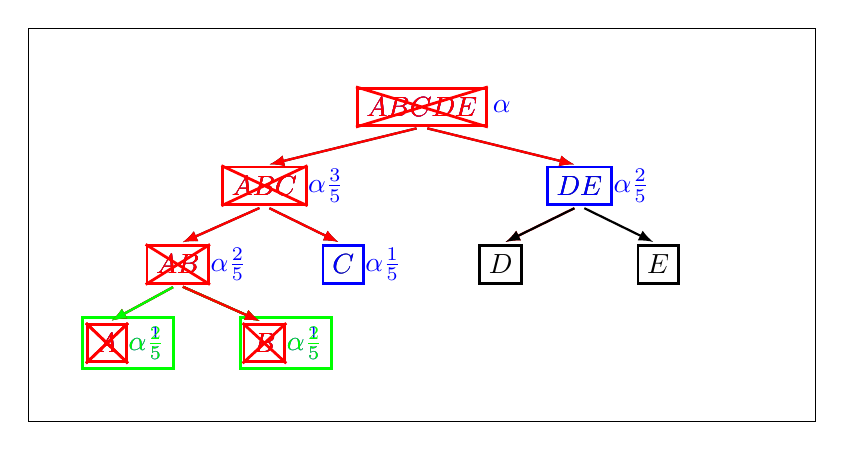
\begin{tikzpicture}
  \draw (0,-1) rectangle (10,4);
  \begin{scope}[draw, line width=1pt]
    \path<1>   [blue]       (5,3) node[draw] (top) {$ABCDE$} ;
  \path<1>[blue]    (top.east)   node {$\quad \alpha$} ;
  \path<2>[blue] (5,3) node[draw] (top) {$ABCDE$} ;
  \path<2->[red] (5,3) node[draw, cross out] (top) {$ABCDE$} ;
  \path<2->[red] (5,3) node[draw] (top) {$ABCDE$} ;
  \path<1-2>     (3,2)  node[draw] (abc) {$ABC$} ;
  \path<2>[blue] (3,2)  node[draw] (abc) {$ABC$} ;
  \path<2>[blue] (abc.east)  node {$\ \quad \alpha \frac{3}{5}$} ;
  \path<3->[red] (3,2) node[draw, cross out] (abc) {$ABC$} ;
  \path<3->[red] (3,2) node[draw] (abc) {$ABC$} ;
  \path<1-2>     (7,2) node[draw] (de) {$DE$} ;
  \path<2->[blue] (7,2) node[draw] (de) {$DE$} ;
  \path<2->[blue] (de.east) node {$\ \quad \alpha \frac{2}{5}$} ;
  \path<1-3>     (1.9,1) node[draw] (ab) {$AB$} ;
  \path<4>[blue] (1.9,1) node[draw] (ab) {$AB$} ;
  \path<4>[blue] (ab.east) node {$\ \quad  \alpha \frac{2}{5}$} ;
  \path<5->[red] (1.9,1) node[draw, cross out] {$AB$} ;
  \path<5->[red] (1.9,1) node[draw] {$AB$} ;
  \path<1-3>     (4,1) node[draw] (c) {$C$} ;
  \path<4->[blue] (4,1) node[draw] (c) {$C$} ;
  \path<4->[blue] (c.east) node {$\ \quad \alpha \frac{1}{5}$} ;
  \path          (6,1) node[draw] (d) {$D$} ;
  \path           (8,1) node[draw] (e) {$E$} ;
  \path     (1,0) node[draw] (a) {$A$};
  \path<5>[blue] (1,0) node[draw] (a) {$A$};
  \path<6>[red]  (1,0) node[draw] (a) {$A$};
  \path<6>[red]  (1,0) node[draw, cross out] (a) {$A$};
  \path<7>[blue] (1,0) node[draw] (a) {$A$};
  \path<8>[red]  (1,0) node[draw] (a) {$A$};
  \path<8>[red]  (1,0) node[draw, cross out] (a) {$A$};
  \path<5>[blue] (a.east)node {$\ \quad \alpha \frac{1}{5}$} ;
  \path<7>[green](a.east)node[draw] {$\ \quad \alpha \frac{2}{5}$} ;
  \path            (3,0) node[draw] (b) {$B$};
  \path<5->[blue]   (3,0) node[draw] (b) {$B$};
  \path<5-6>[blue]  (b.east) node {$\ \quad \alpha \frac{1}{5}$} ;
  \path<7>[green]    (b.east)node[draw] {$\ \quad  \alpha \frac{2}{5}$} ;
  \path<8->[red]    (3,0) node[draw] (b) {$B$};
  \path<8->[red]    (3,0) node[draw, cross out] (b) {$B$};
  \end{scope}
  \begin{scope}[thick, shorten >= 2pt,shorten <= 2pt, latex-]
    \draw         (abc.north) -- (top.south);
    \draw<2->[red] (abc.north) -- (top.south);
    \draw         (de.north) -- (top.south);
    \draw<2>[red] (de.north) -- (top.south);
    \draw         (ab.north) -- (abc.south);
    \draw<4->[red] (ab.north) -- (abc.south);
    \draw (c.north) -- (abc.south);
    \draw<4>[red] (c.north) -- (abc.south);
    \draw (b.north) -- (ab.south);
    \draw (a.north) -- (ab.south);
    \draw (b.north) -- (ab.south);
    \draw<5-6, 8>[red] (a.north) -- (ab.south);
    \draw<5>[red] (b.north) -- (ab.south);
        \draw<7>[green] (a.north) -- (ab.south);
    \draw<7>[green] (b.north) -- (ab.south);
        \draw<8>[red] (b.north) -- (ab.south);
    \draw<4->[red] (d.north) -- (de.south);
    \draw (e.north) -- (de.south);
    \draw (d.north) -- (de.south);
  \end{scope}
  \end{tikzpicture}
\end{figure}
\end{frame}
%%% ==========================

\subsection{}
\begin{frame}
\frametitle{Inheritance procedure (Goeman \& Finos 2009)}

\begin{overprint}
 \onslide<1-6>\bb{}{
   Perform Meinshausen's procedure}\eb
  \onslide<7>
    \bb{}{All leaf nodes in $AB$ are rejected }\eb
      \onslide<8>\bb{}{
    $\frac{2}{5}\alpha$ from $AB$ is \textcolor{green}{inherited} to $C$ (i.e. the closest relative)\\
    test $C$ at $(\frac{1}{5} + \textcolor{green}{\frac{2}{5}})\alpha$}\eb
      \onslide<9>\bb{}{
   suppose $p_C\leq \frac{3}{5}\alpha$}\eb
      \onslide<10>\bb{}{
$\frac{3}{5}\alpha$ from $C$ is \textcolor{green}{inherited} to $DE$}\eb
\end{overprint}

\begin{figure}
  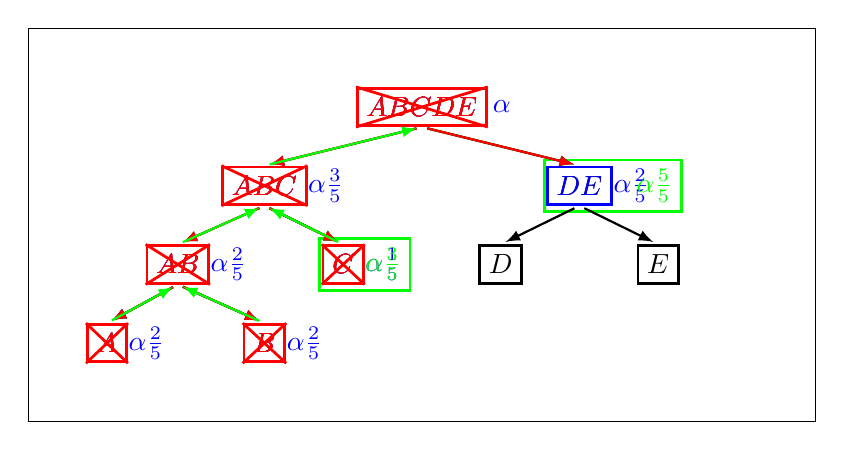
\begin{tikzpicture}
  \draw (0,-1) rectangle (10,4);
  \begin{scope}[draw, line width=1pt]
  \path          (5,3) node[draw] (top) {$ABCDE$} ;
  \path<2>[blue]    (top.east)   node {$\quad \alpha$} ;
  \path<2>[blue] (5,3) node[draw] (top) {$ABCDE$} ;
  \path<3->[red] (5,3) node[draw] (top) {$ABCDE$} ;
  \path<3->[red] (5,3) node[draw,cross out] (top) {$ABCDE$} ;
  \path<1-2>     (3,2)  node[draw] (abc) {$ABC$} ;
  \path<3>[blue] (3,2)  node[draw] (abc) {$ABC$} ;
  \path<3>[blue] (abc.east)node {$\ \quad \alpha \frac{3}{5}$} ;
  \path<4->[red] (3,2) node[draw] (abc) {$ABC$} ;
  \path<4->[red] (3,2) node[draw,cross out] (abc) {$ABC$} ;
  \path<1-2>     (7,2) node[draw] (de) {$DE$} ;
  \path<3->[blue] (7,2) node[draw] (de) {$DE$} ;
  \path<3-9>[blue] (de.east)node {$\ \quad \alpha \frac{2}{5}$} ;
  \path<10->[green] (de.east)node[draw] {$\quad \qquad \alpha \frac{5}{5}$} ;
  \path<1-4>     (1.9,1) node[draw] (ab) {$AB$} ;
  \path<5>[blue] (1.9,1) node[draw] (ab) {$AB$} ;
  \path<5>[blue] (ab.east)node {$\ \quad \alpha \frac{2}{5}$} ;
  \path<6->[red] (1.9,1) node[draw] (ab) {$AB$} ;
  \path<6->[red] (1.9,1) node[draw,cross out] (ab) {$AB$} ;
  \path<1-4>     (4,1) node[draw] (c) {$C$} ;
  \path<5->[blue] (4,1) node[draw] (c) {$C$} ;
  \path<9->[red] (4,1) node[draw] (c) {$C$} ;
  \path<9->[red] (4,1) node[draw,cross out] (c) {$C$} ;
  \path<5-7>[blue] (c.east)node {$\ \quad \alpha \frac{1}{5}$} ;
  \path<8>[green] (c.east)node[draw] {$\ \quad \alpha \frac{3}{5}$} ;
  \path          (6,1) node[draw] (d) {$D$} ;
  \path           (8,1) node[draw] (e) {$E$} ;
  \path     (1,0) node[draw] (a) {$A$};
  \path<6>[blue] (1,0) node[draw] (a) {$A$};
  \path<7->[red]  (1,0) node[draw] (a) {$A$};
  \path<7->[red]  (1,0) node[draw,cross out] (a) {$A$};
  \path<6>[blue] (a.east)node {$\ \quad \alpha \frac{2}{5}$} ;
  \path            (3,0) node[draw] (b) {$B$};
  \path<6>[blue]   (3,0) node[draw] (b) {$B$};
  \path<7->[red]    (3,0) node[draw] (b) {$B$};
  \path<7->[red]    (3,0) node[draw,cross out] (b) {$B$};
    \path<6>[blue] (b.east)node {$\ \quad \alpha \frac{2}{5}$} ;
  \end{scope}
  \begin{scope}[thick, shorten >= 2pt,shorten <= 2pt, latex-]
    \draw<1-9>     (abc.north) -- (top.south);
    \draw<3-9>[red] (abc.north) -- (top.south);
    \draw<10>[green](top.south) -- (abc.north);
    \draw<10>[green](de.north) --(top.south) ;
    \draw<1-9>         (de.north) -- (top.south);
    \draw<3>[red] (de.north) -- (top.south);
    \draw<1-7>         (ab.north) -- (abc.south);
    \draw<5-7, 9->[red] (ab.north) -- (abc.south);
    \draw<8>[green] (abc.south) -- (ab.north);
    \draw<5>[red] (c.north) -- (abc.south);
    \draw<1-4> (c.north) -- (abc.south);
    \draw<6-7> (c.north) -- (abc.south);
    \draw<8>[green] (c.north) --(abc.south) ;
     \draw<9>[red] (c.north) --(abc.south) ;
    \draw<10>[green] (abc.south) --(c.north) ;
    \draw <1-7>(b.north) -- (ab.south);
    \draw <1-7>(a.north) -- (ab.south);
    \draw<1-7> (a.north) -- (ab.south);
    \draw<1-7> (b.north) -- (ab.south);
    \draw<6-7, 9->[red] (a.north) -- (ab.south);
    \draw<6-7, 9->[red] (b.north) -- (ab.south);
    \draw<8>[green] (ab.south) -- (a.north);
    \draw<8>[green] (ab.south) -- (b.north);
    \draw (d.north) -- (de.south);
    \draw (e.north) -- (de.south);
  \end{scope}
  \end{tikzpicture}
\end{figure}

\end{frame}
%%%%%%%%%%%%%%%%%%%%%%%%%%%%
\subsection{Application: Genomics}

\begin{frame}
\frametitle{Microarray-based comparative genomic hybridization (aCGH) Modena et al., 2006 }
  \bb{Data}
    \bi
    \item 2 samples: \\
{\it infratentorial} tumors (14 patients) versus \\ {\it supratentorial} tumors (8 patients). 
 \item chromosome 9 (147 probes)
    \ei
  \eb
  \bb{Inference}
    \begin{itemize}
      \item for each probe (univariate): two sample t-test
      \item The signal is very weak and sparse among probes: \\
      Holm ($\alpha = .05$): no rejections
    \end{itemize}
  \eb
\end{frame}


%%%%%%%%%%%%%%%%%%%%%%%%
\bfr{Results: Inheritance}
\includegraphics[scale=.33]{Modena_ch9}

Significant differences ($\alpha = .05$):
\bb{}
  \rbf{-$\circ$} arm: p 
    \\\rbf{---$\circ$} band: p22.1 and p.21.3
    \\\rbf{-----$\circ$} gene: CTD 2097k16
\eb
\end{frame}
%%================================
\subsection{}
\begin{frame}[fragile]
\frametitle{Software (bioconductor.org)}

\bb{Inheritance procedure}
R package \emph{globaltest}\\
Authors: Goeman \& Finos
\eb
  
\begin{verbatim}
> library(globaltest)
> inheritance()

\end{verbatim}  

\end{frame}

% %==========================DISCUSSION
% %\section{Discussion}
% \subsection{}
% \bfr{Take-home message}
% 
% \bb{Inheritance procedure}
%   \bi 
%     \item Allows inference on tree-structured hypotheses
%     \item Improves Meinshausen
%     \item Available in the R package \emph{globaltest}
% 	\ei
% \eb
% 
% \bb{Future work}
%     \bi 
%     \item Extend to general graphs
%     \item Take into account the dependence between tests
%      \ei
% \eb
% 
% \end{frame}
% =====================================APPLICATION
% \subsection{Application: Genomics}

%%%%%%%%%%%%%%%%%%%%%%%%%%%%%%%%%%%%%%%%%%%%%%%%%%%%%%%%%%%%%%%%%%%%%%%%%%%%%%%%%%%%%%%%%%%%%%%%%%%%%%
\subsection{Application: Neurotoxicity assay}
% \subsection{}
\begin{frame}
\frametitle{Neurotoxicity screening assay (FOB; Moser, 1989)}

\textcolor{cambridgedarkorange}{Goal:} Evaluation of neurotoxic effects of perchlorethylene \\

\bigskip

\textcolor{cambridgedarkorange}{Data:} The United States Enviromental Protection Agency published a guideline (FOB) to assess behavioural and neurologic functions in rats

\begin{itemize}
\item  \textcolor{cambridgedarkblue}{treatment} (1.5g/kg exposure level) versus  \textcolor{cambridgedarkblue}{control} (no exposure)
\item  \textcolor{cambridgedarkblue}{8 rats} at each group
\item  \textcolor{cambridgedarkblue}{21 endpoints} encompassing a wide spectrum of neurologic effects, grouped into  \textcolor{cambridgedarkblue}{6 domains}
\item at each endpoint, the response is \textcolor{cambridgedarkblue}{ordinal} on a scale from \\
1 (absence of adverse effect) to 4 (most severe reaction)
\end{itemize}


\bigskip
\textcolor{cambridgedarkorange}{Challenging statistical problem:} A large number of outcomes for a small sample of subjects

\end{frame}
%%%%%%%%%%%%%%%%%%%%%%%%%%%%%%%%%%%%%%%%%%%%%%%%%%%%%%%%%%%%%%%%%%%%%%%%%%%%%%%%%%%%%%%%%%%%%%%%%%%%%%
\subsection{}
\begin{frame}
\frametitle{Data}

\begin{table}[h!]
\footnotesize
\renewcommand{\tabcolsep}{0.5pc} % enlarge column spacing
\renewcommand{\arraystretch}{.6} % enlarge line spacing
\centering
\begin{tabular}{lll l cccc c cccc}
%\toprule
&Domain & & Endpoint & \multicolumn{9}{c}{Exposure (g/kg)}\\
       &&         && \multicolumn{4}{c}{0 (control)}   &&
       \multicolumn{4}{c}{1.5 (treatment)}\\
\cmidrule{5-8}\cmidrule{10-13}
          &             &
&& 1 & 2 & 3 & 4 && 1 & 2 & 3 & 4  \\
\cmidrule{5-8}\cmidrule{10-13}

&\textcolor{cambridgedarkblue}{Autonomic}

&& \textcolor{cambridgedarkorange}{Lacrimation} &   8   &   0   &   0   &  0  &&
                  5   &   0   &   3   &  0\\

&&&\textcolor{cambridgedarkorange}{Pupil } &        7   &   0   &   1   &  0  &&
                  5   &   0   &   3   &  0\\

&&&\textcolor{cambridgedarkorange}{Defecation} &    7   &   0   &   0   &  1  &&
                  7   &   1   &   0   &  0\\

&&&\textcolor{cambridgedarkorange}{Urination} &     4   &   3   &   1   &  0  &&
                  6   &   1   &   1   &  0\\
                  
                  \midrule

&\textcolor{cambridgedarkblue}{Sensorimotor}

&& \textcolor{cambridgedarkorange}{Approach}  &   8   &   0   &   0   &  0  &&
                 4   &   0   &   3   &  1\\

&&& \textcolor{cambridgedarkorange}{Click}  &       7   &   0   &   1   &  0  &&
                  7   &   0   &   1   &  0\\

&&& \textcolor{cambridgedarkorange}{Tail pinch}  &   6   &   0   &   2   &  0  &&
                   5   &   0   &   3   &  0\\

&&& \textcolor{cambridgedarkorange}{Touch}  &       8   &   0   &   0   &  0  &&
                  6   &   0   &   0   &  2\\

                  \midrule

&\textcolor{cambridgedarkblue}{CNS excitability}


&& \textcolor{cambridgedarkorange}{Handling}  &       6   &   2   &   0   &  0  &&
                     4   &   4   &   0   &  0\\

&&& \textcolor{cambridgedarkorange}{Clonic} &       4   &   4   &   0   &  0  &&
                  5   &   3   &   0   &  0\\

&&& \textcolor{cambridgedarkorange}{Arousal}  &     4   &   3   &   1   &  0  &&
                  3   &   0   &   3   &  2\\

&&& \textcolor{cambridgedarkorange}{Removal}  &       0   &   8   &   0   &  0  &&
                     0   &   7   &   1   &  0\\
                     
                                       \midrule
                     
&\textcolor{cambridgedarkblue}{CNS activity}

&& \textcolor{cambridgedarkorange}{Posture}  &       8   &   0   &   0   &  0  &&
                  7   &   0   &   1   &  0\\

&&& \textcolor{cambridgedarkorange}{Rearing} &      5   &   2   &   1   &  0  &&
                  4   &   2   &   2   &  0\\

                  \midrule

&\textcolor{cambridgedarkblue}{Neuromuscolar}

&& \textcolor{cambridgedarkorange}{Gait}&      8   &   0   &   0   &  0  &&
              3   &   5   &   0   &  0\\

&&& \textcolor{cambridgedarkorange}{Foot splay} &      6   &   1   &   1   &  0  &&
              6   &   1   &   1   &  0\\

&&& \textcolor{cambridgedarkorange}{Forelimb}  &      5   &   2   &   1   &  0  &&
              2   &   1   &   0   &  5\\

&&& \textcolor{cambridgedarkorange}{Hindlimb}  &      5   &   3   &   0   &  0  &&
              0   &   6   &   1   &  1\\

&&& \textcolor{cambridgedarkorange}{Righting}  &      8   &   0   &   0   &  0  &&
              5   &   2   &   1   &  0\\

                  \midrule

&\textcolor{cambridgedarkblue}{Psysicological}

&& \textcolor{cambridgedarkorange}{Weight} &      6   &   1   &   1   &  0  &&
              4   &   2   &   0   &  2\\

&&& \textcolor{cambridgedarkorange}{Temperature}  &      6   &   1   &   1   &  0  &&
                        4   &   3   &   0   &  1\\

%\bottomrule
\end{tabular}
\end{table}


\end{frame}
%%%%%%%%%%%%%%%%%%%%%%%%%%%%%%%%%%%%%%%%%%%%%%%%%%%%%%%%%%%%%%%%%%%%%%%%%%%%%%%%%%%%%%%%%%%%%%%%%%%%%%
\subsection{}
\begin{frame}
\frametitle{Multiple hypotheses}
$$H:  \textcolor{cambridgedarkorange}{Y_{H}} \stackrel{\mathrm{d}}{=} \textcolor{cambridgedarkblue}{X_{H}}\quad \mathrm{versus}\quad \tilde{H}:  \textcolor{cambridgedarkorange}{Y_{H}} \stackrel{\mathrm{st}}{\gneq} \textcolor{cambridgedarkblue}{X_{H}},\qquad H\in \mathcal{H}$$

\includegraphics[scale=.38]{endpoints}

\end{frame}
%%%%%%%%%%%%%%%%%%%%%%%%%%%%%%%%%%%%%%%%%%%%%%%%%%%%%%%%%%%%%%%%%%%%%%%%%%%%%%%%%%%%%%%%%%%%%%%%%%%%%%
% \subsection{}
% \begin{frame}
% \frametitle{Marginal stochastic order model}
% 
% 
% \begin{columns}[t]
% 
% \column{0.55\textwidth}
% 
% $\mathbf{X}=
% (X_A,X_B)\sim \mathrm{Multinomial}(\{\omega_{A,B}(i,j)\})$
% 
% \bigskip
% 
% \begin{tikzpicture}
% \foreach \x in {0,.5,1,1.5}
% \foreach \y in {0,.5,1,1.5}
% {
% \draw (\x,\y) +(-.25,-.25) rectangle ++(.25,.25);
% \draw[color=cambridgedarkorange]  (\x,-1) +(-.25,-.25) rectangle ++(.25,.25);
% \draw[color=cambridgedarkorange] (2.5,\y) +(-.25,-.25) rectangle ++(.25,.25);
% \draw (2.5,-1) +(-.25,-.25) rectangle ++(.25,.25);
% }
% \node at (2.5,2) {$\omega_A$};
% \node at (-.75,-1) {$\omega_B$};
% \node at (-.75,2) {$\omega_{A,B}$};
% \node at (2.5,-1) {$1$};
% \end{tikzpicture}
% 
% \column{0.55\textwidth}
% 
% $\mathbf{Y}=(Y_A,Y_B)\sim \mathrm{Multinomial}(\{\tau_{A,B}(i,j)\})$
% 
% \bigskip
% 
% \begin{tikzpicture}
% \foreach \x in {0,.5,1,1.5}
% \foreach \y in {0,.5,1,1.5}
% {
% \draw (\x,\y) +(-.25,-.25) rectangle ++(.25,.25);
% \draw[color=cambridgedarkorange]  (\x,-1) +(-.25,-.25) rectangle ++(.25,.25);
% \draw[color=cambridgedarkorange]  (2.5,\y) +(-.25,-.25) rectangle ++(.25,.25);
% \draw (2.5,-1) +(-.25,-.25) rectangle ++(.25,.25);
% }
% \node at (2.5,2) {$\tau_A$};
% \node at (-.75,-1) {$\tau_B$};
% \node at (-.75,2) {$\tau_{A,B}$};
% \node at (2.5,-1) {$1$};
% \end{tikzpicture}
% 
% \end{columns}
% 
% \bigskip
% 
% 
% $$\mathcal{M}_{\mathrm{M}}=\left\{ \begin{array}{cc}
%     X_{A}\stackrel{\mathrm{st}}{\leq}Y_{A}: &  \sum_{i=1}^{k}\omega_{A}(i)\geq \sum_{i=1}^{k}\tau_{A}(i), k=1,\ldots,4 \\ 
%     X_{B}\stackrel{\mathrm{st}}{\leq}Y_{B}: &  \sum_{j=1}^{l}\omega_{B}(j)\geq \sum_{j=1}^{k}\tau_{B}(j), l=1,\ldots,4 \\ 
%     \end{array}\right\}$$
% 
% \end{frame}
% %%%%%%%%%%%%%%%%%%%%%%%%%%%%%%%%%%%%%%%%%%%%%%%%%%%%%%%%%%%%%%%%%%%%%%%%%%%%%%%%%%%%%%%%%%%%%%%%%%%%%%
% \subsection{}
% \begin{frame}
% \frametitle{Marginal null model}
% 
% 
% \begin{columns}[t]
% 
% \column{0.55\textwidth}
% 
% $\mathbf{X}=(X_A,X_B)\sim \mathrm{Multinomial}(\{\omega_{A,B}(i,j)\})$
% 
% \bigskip
% 
% \begin{tikzpicture}
% \foreach \x in {0,.5,1,1.5}
% \foreach \y in {0,.5,1,1.5}
% {
% \draw (\x,\y) +(-.25,-.25) rectangle ++(.25,.25);
% \draw[color=cambridgedarkorange] (\x,-1) +(-.25,-.25) rectangle ++(.25,.25);
% \draw[color=cambridgedarkorange]   (2.5,\y) +(-.25,-.25) rectangle ++(.25,.25);
% \draw   (2.5,-1) +(-.25,-.25) rectangle ++(.25,.25);
% \draw (\x,\y) node{\tiny{$1/16$}};
% \draw[color=cambridgedarkorange]  (\x,-1) node{\tiny{$1/4$}};
% \draw[color=cambridgedarkorange]  (2.5,\y) node{\tiny{$1/4$}};
% }
% \node at (2.5,2) {$\omega_A$};
% \node at (-.75,-1) {$\omega_B$};
% \node at (-.75,2) {$\omega_{A,B}$};
% \node at (2.5,-1) {$1$};
% \end{tikzpicture}
% 
% \bigskip
% 
% $\qquad\lambda_{A}$: independence
% 
% \column{0.55\textwidth}
% 
% $\mathbf{Y}=(Y_A,Y_B)\sim \mathrm{Multinomial}(\{\tau_{A,B}(i,j)\})$
% 
% \bigskip
% 
% \begin{tikzpicture}
% \foreach \x in {0,.5,1,1.5}
% \foreach \y in {0,.5,1,1.5}
% {
% \draw (\x,\y) +(-.25,-.25) rectangle ++(.25,.25);
% \draw[color=cambridgedarkorange]   (\x,-1) +(-.25,-.25) rectangle ++(.25,.25);
% \draw[color=cambridgedarkorange]   (2.5,\y) +(-.25,-.25) rectangle ++(.25,.25);
% \draw (2.5,-1) +(-.25,-.25) rectangle ++(.25,.25);
% \draw[color=cambridgedarkorange]  (\x,-1) node{\tiny{$1/4$}};
% \draw[color=cambridgedarkorange]  (2.5,\y) node{\tiny{$1/4$}};
% \draw (1.5,0) node{\tiny{$1/4$}};
% \draw (1,.5) node{\tiny{$1/4$}};
% \draw (.5,1) node{\tiny{$1/4$}};
% \draw (0,1.5) node{\tiny{$1/4$}};
% }
% \node at (2.5,2) {$\tau_A$};
% \node at (-.75,-1) {$\tau_B$};
% \node at (-.75,2) {$\tau_{A,B}$};
% \node at (2.5,-1) {$1$};
% \end{tikzpicture}
% 
% \bigskip
% 
% $\quad\lambda_{B}$: complete dependence
% 
% \end{columns}
% 
% \bigskip
% 
% 
% $$\mathcal{M}_{\mathrm{M}_{0}}=\left\{ \begin{array}{cc}
%     X_{A}\stackrel{\mathrm{d}}{=}Y_{A}: &  \omega_{A}(i)=\tau_{A}(i), i=1,\ldots,4 \\ 
%     X_{B}\stackrel{\mathrm{d}}{=}Y_{B}: &  \omega_{B}(j)=\tau_{B}(j), j=1,\ldots,4 \\ 
% \end{array}\right\}$$
% 
% 
% 
% \end{frame}
% %%%%%%%%%%%%%%%%%%%%%%%%%%%%%%%%%%%%%%%%%%%%%%%%%%%%%%%%%%%%%%%%%%%%%%%%%%%%%%%%%%%%%%%%%%%%%%%%%%%%%%
% \begin{frame}
% \frametitle{Marginal exchangeability}
% 
% $\mathbf{X}_{r}=(X_{A,r},X_{B,r})^t,r=1,\ldots,8,\stackrel{\mathrm{i.i.d.}}\sim\mathbf{X}$  control sample\\
% $\mathbf{Y}_{r}=(Y_{A,r},Y_{B,r})^t,r=1,\ldots,8, \stackrel{\mathrm{i.i.d.}}\sim \mathbf{Y}$ treatment sample
% $(\mathbf{Z}_{1},\ldots,\mathbf{Z}_{16}) = (\mathbf{X}_{1},\ldots,\mathbf{X}_{8},\mathbf{Y}_{1},\ldots,\mathbf{Y}_{8})$ pooled sample
% 
% \bigskip
% 
% Under $\mathcal{M}_{\mathrm{M}_0}$,
% 
% $$(Z_{A,1},\ldots,Z_{A,16}) \stackrel{\mathrm{d}}{=}(Z_{A,\pi(1)},\ldots,Z_{A,\pi(16)})$$
% $$(Z_{B,1},\ldots,Z_{B,16})  \stackrel{\mathrm{d}}{=}( Z_{B,\pi'(1)},\ldots,Z_{B,\pi'(16)})$$
% 
% \bigskip
% 
% but in general
% 
% $$\left( \left(\begin{array}{c}
%     Z_{A,1} \\ 
%     Z_{B,1} \\ 
%   \end{array}\right),\ldots, \left(  \begin{array}{c}
%     Z_{A,16} \\ 
%     Z_{B,16} \\ 
%   \end{array}\right) \right)  \stackrel{\mathrm{d}}{\neq} \left(\left(\begin{array}{c}
%     Z_{A,\pi(1)} \\ 
%     Z_{B,\pi(1)} \\ 
%   \end{array}\right),\ldots, \left(  \begin{array}{c}
%     Z_{A,\pi(16)} \\ 
%     Z_{B,\pi(16)} \\ 
%   \end{array}\right)\right)$$
%  
% 
% %no information about the joint distribution of $\mathbf{Z}=
% %\left(  \begin{array}{c}
% %    Z_A \\ 
% %    Z_B \\ 
% %  \end{array}\right)$
% 
% %$\Pr(\mathbf{Z}_{1},\ldots,\mathbf{Z}_{16}) = \Pr(Z_{A,\pi(1)},\ldots,Z_{A,\pi(16)}) = 1/16!$
% 
% 
% 
% \end{frame}
% %%%%%%%%%%%%%%%%%%%%%%%%%%%%%%%%%%%%%%%%%%%%%%%%%%%%%%%%%%%%%%%%%%%%%%%%%%%%%%%%%%%%%%%%%%%%%%%%%%%%%%
% %%%%%%%%%%%%%%%%%%%%%%%%%%%%%%%%%%%%%%%%%%%%%%%%%%%%%%%%%%%%%%%%%%%%%%%%%%%%%%%%%%%%%%%%%%%%%%%%%%%%%%
% \subsection{}
% \begin{frame}
% \frametitle{Joint null model (no effect)}
% 
% 
% \begin{columns}[t]
% 
% \column{0.55\textwidth}
% 
% $\mathbf{X}=(X_A,X_B)\sim \mathrm{Multinomial}(\{\omega_{A,B}(i,j)\})$
% 
% \bigskip
% 
% \begin{tikzpicture}
% \foreach \x in {0,.5,1,1.5}
% \foreach \y in {0,.5,1,1.5}
% {
% \draw[color=cambridgedarkorange]   (\x,\y) +(-.25,-.25) rectangle ++(.25,.25);
% \draw (\x,-1) +(-.25,-.25) rectangle ++(.25,.25);
% \draw (2.5,\y) +(-.25,-.25) rectangle ++(.25,.25);
% \draw (2.5,-1) +(-.25,-.25) rectangle ++(.25,.25);
% \draw[color=cambridgedarkorange]   (\x,\y) node{\tiny{$\lambda$}};
% }
% \node at (2.5,2) {$\omega_A$};
% \node at (-.75,-1) {$\omega_B$};
% \node at (-.75,2) {$\omega_{A,B}$};
% \node at (2.5,-1) {$1$};
% \end{tikzpicture}
% 
% 
% 
% \column{0.55\textwidth}
% 
% $\mathbf{Y}=(Y_A,Y_B)\sim \mathrm{Multinomial}(\{\tau_{A,B}(i,j)\})$
% 
% \bigskip
% 
% \begin{tikzpicture}
% \foreach \x in {0,.5,1,1.5}
% \foreach \y in {0,.5,1,1.5}
% {
% \draw[color=cambridgedarkorange] (\x,\y) +(-.25,-.25) rectangle ++(.25,.25);
% \draw (\x,-1) +(-.25,-.25) rectangle ++(.25,.25);
% \draw (2.5,\y) +(-.25,-.25) rectangle ++(.25,.25);
% \draw (2.5,-1) +(-.25,-.25) rectangle ++(.25,.25);
% \draw[color=cambridgedarkorange] (\x,\y) node{\tiny{$\lambda$}};
% }
% \node at (2.5,2) {$\tau_A$};
% \node at (-.75,-1) {$\tau_B$};
% \node at (-.75,2) {$\tau_{A,B}$};
% \node at (2.5,-1) {$1$};
% \end{tikzpicture}
% 
% 
% 
% 
% \end{columns}
% 
% \bigskip
% 
% $\qquad\qquad\qquad\quad\quad\lambda$: any form of dependence
% 
% \bigskip
% 
% 
% $$\mathcal{M}_{\mathrm{J}_{0}}=\left\{ \begin{array}{cc}
%     \mathbf{X}\stackrel{\mathrm{d}}{=}\mathbf{Y}: &  \omega_{A,B}(i,j)=\tau_{A,B}(i,j) \,\, \forall\,(i,j)
% \end{array}\right\}\subset \mathcal{M}_{\mathrm{M}_{0}}$$
% 
% 
% 
% \end{frame}
% %%%%%%%%%%%%%%%%%%%%%%%%%%%%%%%%%%%%%%%%%%%%%%%%%%%%%%%%%%%%%%%%%%%%%%%%%%%%%%%%%%%%%%%%%%%%%%%%%%%%%%
% \begin{frame}
% \frametitle{Joint exchangeability}
% 
% 
% 
% Under $\mathcal{M}_{\mathrm{J}_0}$,
% 
% $$(\mathbf{Z}_{1},\ldots,\mathbf{Z}_{16}) \stackrel{\mathrm{d}}{=} (\mathbf{Z}_{\pi(1)},\ldots,\mathbf{Z}_{\pi(16)})$$
% 
% 
% \bigskip
% 
% the conditional critical region of $S_{\max}$ is similar
% 
% $$\Pr(S_{\max} > c|(\mathbf{z}_{1},\ldots,\mathbf{z}_{16}); \lambda) = \frac{\sum_{b=1}^{16!} I\{S_{\max}\circ \pi_b > c\}}{16!}\quad \forall\, \lambda\in \mathcal{M}_{\mathrm{J}_{0}}$$
% 
% \bigskip
% 
% single-step and monotonicity conditions fulfilled $\Rightarrow$ FWE control (exact)
% 
% 
% 
% \end{frame}
% %%%%%%%%%%%%%%%%%%%%%%%%%%%%%%%%%%%%%%%%%%%%%
% %%%%%%%%%%%%%%%%%%%%%%%%%%%%%%%%%%%%%%%%%%%%%
% \subsection{}
% \begin{frame}
% \frametitle{Joint stochastic order model}
% 
% 
% \begin{columns}[t]
% 
% \column{0.55\textwidth}
% 
% $\mathbf{X}=(X_A,X_B)\sim \mathrm{Multinomial}(\{\omega_{A,B}(i,j)\})$
% 
% \bigskip
% 
% \begin{tikzpicture}
% \foreach \x in {0,.5,1,1.5}
% \foreach \y in {0,.5,1,1.5}
% {
% \draw  (\x,\y) +(-.25,-.25) rectangle ++(.25,.25);
% \draw (\x,-1) +(-.25,-.25) rectangle ++(.25,.25);
% \draw (2.5,\y) +(-.25,-.25) rectangle ++(.25,.25);
% \draw (2.5,-1) +(-.25,-.25) rectangle ++(.25,.25);
% }
% \node at (2.5,2) {$\omega_A$};
% \node at (-.75,-1) {$\omega_B$};
% \node at (-.75,2) {$\omega_{A,B}$};
% \node at (2.5,-1) {$1$};
% \only<1>{\draw[color=cambridgedarkorange] (1,1.5) node{\tiny{$U$}};
% \draw[color=cambridgedarkorange] (1.5,1.5) node{\tiny{$U$}};
% \draw[color=cambridgedarkorange] (1.5,1) node{\tiny{$U$}};
% \draw[color=cambridgedarkorange] (1,1) node{\tiny{$U$}};
% }
% \only<2>{\draw[color=cambridgedarkorange] (1,1.5) node{\tiny{$U$}};
% \draw[color=cambridgedarkorange] (1.5,1.5) node{\tiny{$U$}};
% \draw[color=cambridgedarkorange] (1.5,1) node{\tiny{$U$}};
% \draw[color=cambridgedarkorange] (.5,1.5) node{\tiny{$U$}};
% \draw[color=cambridgedarkorange] (1.5,0.5) node{\tiny{$U$}};
% }
% \end{tikzpicture}
% 
% \column{0.55\textwidth}
% 
% $\mathbf{Y}=(Y_A,Y_B)\sim \mathrm{Multinomial}(\{\tau_{A,B}(i,j)\})$
% 
% \bigskip
% 
% \begin{tikzpicture}
% \foreach \x in {0,.5,1,1.5}
% \foreach \y in {0,.5,1,1.5}
% {
% \draw (\x,\y) +(-.25,-.25) rectangle ++(.25,.25);
% \draw (\x,-1) +(-.25,-.25) rectangle ++(.25,.25);
% \draw (2.5,\y) +(-.25,-.25) rectangle ++(.25,.25);
% \draw (2.5,-1) +(-.25,-.25) rectangle ++(.25,.25);
% }
% \node at (2.5,2) {$\tau_A$};
% \node at (-.75,-1) {$\tau_B$};
% \node at (-.75,2) {$\tau_{A,B}$};
% \node at (2.5,-1) {$1$};
% \only<1>{\draw[color=cambridgedarkorange] (1,1.5) node{\tiny{$U$}};
% \draw[color=cambridgedarkorange] (1.5,1.5) node{\tiny{$U$}};
% \draw[color=cambridgedarkorange] (1.5,1) node{\tiny{$U$}};
% \draw[color=cambridgedarkorange] (1,1) node{\tiny{$U$}};
% }
% \only<2>{\draw[color=cambridgedarkorange] (1,1.5) node{\tiny{$U$}};
% \draw[color=cambridgedarkorange] (1.5,1.5) node{\tiny{$U$}};
% \draw[color=cambridgedarkorange] (1.5,1) node{\tiny{$U$}};
% \draw[color=cambridgedarkorange] (.5,1.5) node{\tiny{$U$}};
% \draw[color=cambridgedarkorange] (1.5,0.5) node{\tiny{$U$}};
% }
% \end{tikzpicture}
% 
% \end{columns}
% 
% \bigskip
% 
% 
% $$\mathcal{M}_{\mathrm{J}}=\left\{ \begin{array}{cc}
%     \mathbf{X}\stackrel{\mathrm{st}}{\leq}\mathbf{Y}: &  \sum_{(i,j)\in U}\omega_{A,B}(i,j)\geq  \sum_{(i,j)\in U}\tau_{A,B}(i,j) \,\,\forall\,\,U\in \mathcal{U}
% \end{array}\right\}\subset \mathcal{M}_{\mathrm{M}}$$
% 
% \bigskip
% 
% $U\in \mathcal{U}$ upper set, $|\mathcal{U}|={8 \choose 4}=70$ 
% 
% \end{frame}
% %%%%%%%%%%%%%%%%%%%%%%%%%%%%%%%%
% \subsection{}
% \begin{frame}
% \frametitle{Model assumption}
% 
% \textcolor{cambridgedarkorange}{\textbf{Theorem}\footnote{A. Solari (2007) PhD Thesis; B. Klingenberg et al. (2008)  \emph{Biometrics}}}
% 
% \bigskip
% If the assumed model is $\mathcal{M}_{\mathrm{J}}$,
% 
% $$\mathcal{M}_{\mathrm{J}} \cap \mathcal{M}_{\mathrm{M_{0}}}= \mathcal{M}_{\mathrm{J_{0}}}$$
% 
% Then any permutation-based sequential procedure controls the FWE
% 
% 
% 
% 
% \end{frame}
%%%%%%%%%%%%%%%%%%%%%%%%%%%%%%%%%%%%%%%%%%%%%
%%%%%%%%%%%%%%%%%%%%%%%%%%%%%%%%%%%%%%%%%%%%%
\subsection{}
\begin{frame}
\frametitle{Test statistics}

Ordinal measurement: distances between categories are unknown

Mantel's test $S_H(\mathbf{w})$ depends on nondecreasing scores $\mathbf{w}$ assigned to categories. 

To overcome this problem, consider as the test statistic

$$S^{\max}_{H}=\max_{\mathbf{w}} \{S_{H}(\mathbf{w})\}$$

where $\mathbf{w}^{\max}$ maximizing $S_H(\mathbf{w})$ can be found by isotonic regression (adaptive test)

\begin{columns}[t]
\column{0.5\textwidth}
\bigskip
\begin{tabular}{c|cccc|c}
   Arousal  & I & II & III & IV & \\
 \hline
1.5 g/kg & 2 &  1 & 3 & 2 & 8\\
0 g/kg & 5 & 2 & 1 & 0 & 8 \\
\hline
\end{tabular}
% \bigskip
% 
\only<1> {$\mathbf{w}^{\mathrm{es}}=(0,1/3,2/3,1)$\\
\bigskip

$S_H(\mathbf{w}^{\mathrm{es}})=2.07$
}
\only<2>{$\mathbf{w}^{\max}=(0,0.07,0.65,1)$\\
\bigskip

$S_{H}^{\max}=S_H(\mathbf{w}^{\max})=2.15$
% Use $S_{H}^{\max}\circ\pi$ 
}
\column{0.5\textwidth}

\only<1>{\includegraphics[scale=0.3]{CTperE}}
\only<2>{\includegraphics[scale=0.3]{CTpmM}}


\end{columns}

\end{frame}
%%%%%%%%%%%%%%%%%%%%%%%%%%%%%%%%%%%%%%%%%%%%%%%%%%%%%%%%%%%%%%%%%%%%%%%%%%%%%%%%%%%%%%%%%%%%%%%%%%%%%%
\begin{frame}
\frametitle{Inference}

p-values for Endpoints (i.e. univariate test) are found by permutation approach (i.e. resampling based)

p-values for Domains (i.e. multivariate test) are found by combination of univariate ones (Pesarin 2001, klingenberg et al. 2009)


\end{frame}
%%%%%%%%%%%%%%%%%%%%%%%%%%%%%%%%%%%%%%%%%%%%%%%%%%%%%%%%%%%%%%%%%%%%%%%%%%%%%%%%%%%%%%%%%%%%%%%%%%%%%%
\subsection{}
\begin{frame}
\frametitle{Results: endpoint level}

\only<1>{\includegraphics[scale=0.43]{rawP}

\bigskip

$\odot$ = raw p-values 

}
\only<2>{\includegraphics[scale=0.43]{BonfHolmP}

\bigskip

adjusted p-values: $\odot$ = Inheritance, x = Holm
}

\end{frame}
%%%%%%%%%%%%%%%%%%%%%%%%%%%%%%%%%%%%%%%%%%%%%%%%%%%%%%%%%%%%%%%%%%%%%%%%%%%%%%%%%%%%%%%%%%%%%%%%%%%%%%
\begin{frame}
\frametitle{Results: domain level}

\includegraphics[scale=0.43]{Dom}

\bigskip 

adjusted p-values: $\bigcirc$ = Inheritance

\end{frame}

%%%%%%%%%%%%%%%%%%%%%%%%%%%%%%%%%%%%%%%%%%%%%%%%%%%%%%%%%%%%%%%%%%%%%%%%%%%%%%%%%%%%%%%%%%%%%%%%%%%%%%

%==========================DISCUSSION
%\section{Discussion}
\subsection{}
\bfr{Take-home message}

\bb{Inheritance procedure}
  \bi 
    \item Allows inference on tree-structured hypotheses
    \item Improves Meinshausen
    \item Available in the R package \emph{globaltest}
	\ei
\eb

\bb{Furthermore}
    \bi 
    \item Extention to general graphs
    \item Extention to high dimension
     \ei
\eb

\end{frame}

\bfr{Take-home message}

\bb{Sequential Rejection principle}
\bi
\item A unifying approach, \\
it includes other methods (Shaffer's, fallback, focus level, Meinshausen's, Rosenbaum's, etc.)\\  
Some other FWE controlling procedures do not fit (Sidak, Hochberg)
\item Easy-to-check conditions of FWER control
\item Useful tool to formulate procedures
\ei
\eb
\end{frame}
%(generally require independence of test statistics)

% \bigskip
% 
% \textcolor{cambridgedarkorange}{High-dimensional multiple testing (e.g. genomics, $|\mathcal{H}|=10000$)}
% 
% \begin{itemize}
% \item new methodological and computational challenges
% \item controlling the FWE can be ``playing it too safe''
% \item replace FWE by a more liberal measure (e.g $k$-FWE, FDR, etc.)
% \end{itemize}
% 


%%%%%%%%%%%%%%%%%%%%%%%%%%%%%%%%%%%%%%%%%%%%%%%%%%%%%%%%%%%%%%%%%%%%%%%%%%%%%%%%%%%%%%%%%%%%%%%%%%%%%%
\end{document}
